\documentclass[11pt,reqno]{amsart}

\usepackage[utf8]{inputenc}
\usepackage[T1]{fontenc}
\usepackage{lmodern}
\usepackage{amsmath,amssymb,amsfonts,amsthm,mathtools}
\usepackage{booktabs,array,multirow}
\usepackage{graphicx}
\usepackage{enumitem}
\usepackage[margin=1.0in]{geometry}
\usepackage{microtype}
\usepackage{xcolor}
\definecolor{linkblue}{rgb}{0.0,0.2,0.6}
\usepackage[colorlinks=true,linkcolor=linkblue,citecolor=linkblue,urlcolor=linkblue]{hyperref}

\newtheorem{theorem}{Theorem}[section]
\newtheorem{proposition}[theorem]{Proposition}
\newtheorem{lemma}[theorem]{Lemma}
\newtheorem{corollary}[theorem]{Corollary}
\theoremstyle{definition}
\newtheorem{definition}[theorem]{Definition}
\theoremstyle{remark}
\newtheorem{remark}[theorem]{Remark}

\numberwithin{equation}{section}
\allowdisplaybreaks

\newcommand{\R}{\mathbb{R}}
\newcommand{\C}{\mathbb{C}}
\newcommand{\N}{\mathbb{N}}
\newcommand{\Z}{\mathbb{Z}}
\newcommand{\dd}{\mathrm{d}}
\newcommand{\ee}{\mathrm{e}}
\newcommand{\ii}{\mathrm{i}}
\newcommand{\Rea}{\mathrm{Re}}
\newcommand{\Ima}{\mathrm{Im}}
\newcommand{\Tr}{\mathrm{Tr}}
\newcommand{\sinch}{\mathrm{sinc}_{\mathrm{hyp}}}
\newcommand{\fac}{\mathclose{\mathchar"0021}}

\title[Mother-Wavelet Decomposition and Explicit Remainder Bounds]{Universal Mother-Wavelet Decomposition of the Jacobi--Riemann Kernel, Smooth Jacobi--Sinh Shells, and Explicit Saddle-Point Remainder Bounds for Riemann's $\Xi$-Function}

\author{Thijs Missiaen}
\address{Independent Researcher, Belgium}
\email{thijs.missiaen@gmail.com}
\thanks{ORCID: \href{https://orcid.org/0009-0007-3678-0810}{0009-0007-3678-0810}}

\subjclass[2020]{Primary 11M06, 41A60; Secondary 30D15, 33B15}
\keywords{Riemann $\Xi$-function, transverse Wronskian, Jacobi theta kernel, mother-wavelet dilation, Riemann--Siegel formula, Gabcke remainder bounds, Stieltjes constants, Wigner phase-space shift}
\date{April 2026}

\begin{document}

\begin{abstract}
We establish the harmonic and saddle-point decomposition of the Jacobi--Riemann kernel $\Phi(u) = \sum_{m=1}^{\infty} \phi_m(u)$ governing the transverse Wronskian $W(d,t) = R I_t - I R_t$ of Riemann's $\Xi(t - \ii d) = R + \ii I$. Every shell $\phi_m(u) = m^{-1/2}\varphi_1(u + \frac{1}{2}\ln m)$ is an exact logarithmic translation of a single mother wavelet $\varphi_1(w)$ whose bilateral Laplace--Mellin transform $\mathcal{G}(s) = \frac{1}{8}s(s-1)\pi^{-s/2}\Gamma(s/2)$ exhibits exact polynomial cancellation $|(1-s)(-s)| \equiv |s(s-1)|$ along $s = \frac{1}{2} + d + \ii t$, yielding a three-line reflection-ellipse proof of $W_{1,1}(d,t) > 0$ and the Symmetric Branch-Damping Inequality across all active Riemann--Siegel modes $1 \le n \le N(t) = \lfloor\sqrt{t/2\pi}\rfloor$. Smooth self-mirrored Jacobi--Sinh shells eliminate the $u = 0$ odd-derivative kink of naive half-line truncations, while the diagonal sum $\mathcal{D}_{\mathrm{diag}}(d,t)$ obeys a non-oscillatory $(\ln t)^3$ Stieltjes expansion that dominates both the $\mathcal{O}(t^{-3/2})$ self-damped boundary cross-pair $(N-1,N)$ and explicit incomplete-Gamma and two-dimensional Gabcke--Olver remainder envelopes.
\end{abstract}

\maketitle

\section{Introduction and Main Results}\label{sec:intro}

In his foundational 1859 memoir, Riemann~\cite{riemann1859} introduced the completed zeta function $\xi(s) = \frac{1}{2}s(s-1)\pi^{-s/2}\Gamma(s/2)\zeta(s)$ and its critical-line rotation $\Xi(z) := \xi(\frac{1}{2} + \ii z)$, represented as the Fourier cosine transform of the super-exponentially decaying Jacobi theta kernel~\cite{jacobi1829,polya1926,titchmarsh1986}. Decomposing $\Xi(t - \ii d) = R(d,t) + \ii\,I(d,t)$ for spectral height $t \in \R$ and transverse displacement $d = \sigma - \frac{1}{2} > 0$, the transverse Wronskian $W(d,t) := R(d,t)I_t(d,t) - I(d,t)R_t(d,t) = |\Xi(t - \ii d)|^2 \partial_t \arg \Xi(t - \ii d)$ governs both the vertical monotonicity of $|\Xi(t - \ii d)|^2$ via the Cauchy--Riemann identity $\partial_d(|\Xi|^2) = 2W(d,t)$ and the topological zero-detection criteria of Speiser~\cite{speiser1934}, Hinkkanen~\cite{hinkkanen1997}, and Lagarias~\cite{lagarias1999}.

In Papers~I--IV of this series~\cite{missiaen2026paper1,missiaen2026paper2,missiaen2026paper3,missiaen2026paper4}, the Wronskian $W(d,t)$ was cast into Wigner phase-space coordinates $(x,y) = (u+v, u-v)$~\cite{wigner1932,hudson1974} and analyzed through complex saddle-point coalescence, parity-reduced kernel stiffness, Chladni nodal chamber geometry, and de~Branges--Jensen positivity~\cite{csordas1986}. A central structural problem remains at the bridge between the exact integral representation of $\Xi(z)$ and the finite Riemann--Siegel Dirichlet sum~\cite{siegel1932,gabcke1979,olver1997} of length $N(t) = \lfloor\sqrt{t/2\pi}\rfloor$: how do the individual summation modes $\phi_m(u)$ of the Jacobi--Riemann kernel $\Phi(u) = \sum_{m=1}^{\infty} \phi_m(u)$ interact in the bilinear Wronskian matrix, why does naive half-line shell splitting produce a severe $\mathcal{O}(t^{-2})\ee^{\pi t/2}$ boundary artifact at $u = 0$, why does the slowest adjacent boundary pair $(N-1,N)$ not destabilize the diagonal sum as its frequency gap $\Omega_{\min}(t) = \ln(N/(N-1)) \sim \sqrt{2\pi/t}$ narrows, and how are the infinite saddle-point tails bounded explicitly across the two-dimensional half-strip $\mathcal{S}_{1/2}^+ := \{(d,t) \in (0, 1/2] \times [14, \infty)\}$?

The present paper (Paper~V) resolves these four questions within a unified analytical framework. Our main results are consolidated in the following theorem.

\begin{theorem}[Universal Mother-Wavelet Decomposition, Smooth Jacobi--Sinh Shells, and Explicit Remainder Bounds]\label{thm:main}
Let $\Phi(u) = \sum_{m=1}^{\infty} \phi_m(u)$ with $\phi_m(u) = (2\pi^2 m^4 \ee^{9u} - 3\pi m^2 \ee^{5u})\exp(-\pi m^2 \ee^{4u})$, and let $s = \frac{1}{2} + d + \ii t$ with $z = t - \ii d$. Then the following four structural laws hold:
\begin{enumerate}[label=\textup{(\roman*)},leftmargin=2.2em]
\item \textbf{Universal Mother-Wavelet Dilation and Symmetric Branch Damping.} Every shell $\phi_m(u)$ is an exact logarithmic translation of the mother wavelet $\varphi_1(w) := \phi_1(w)$:
\begin{equation}\label{eq:intro_dilation}
\phi_m(u) = m^{-1/2}\,\varphi_1\!\left(u + \frac{1}{2}\ln m\right) \qquad (m \ge 1,\; u \in \C),
\end{equation}
with bilateral Laplace--Mellin transform $\mathcal{G}(s) := \int_{-\infty}^{\infty} \varphi_1(v)\ee^{2(s-1/2)v}\,\dd v = \frac{1}{8}s(s-1)\pi^{-s/2}\Gamma(s/2)$. Because $|(1-s)(-s)| \equiv |s(s-1)|$ holds identically on $\C$, the polynomial prefactor cancels completely in the reflection modulus ratio $\rho_\Gamma(d,t) := |\mathcal{G}(1-s)/\mathcal{G}(s)| = \pi^d |\Gamma(\frac{1}{4}-\frac{d}{2}+\ii\frac{t}{2})/\Gamma(\frac{1}{4}+\frac{d}{2}+\ii\frac{t}{2})| = \exp(-2\int_0^d \mathcal{A}_\Gamma^{\mathrm{sym}}(u,t)\,\dd u) < 1$ for all $d > 0$ and $t \ge 7 > t_{\mathrm{crit}} = 6.2898359888\dots$. Consequently, $W_{1,1}(d,t) > 0$ and every active mode $1 \le n \le N(t) = \lfloor\sqrt{t/2\pi}\rfloor$ obeys the Symmetric Branch-Damping Inequality:
\begin{equation}\label{eq:intro_branch_damp}
\rho_\Gamma(d,t)\,n^{-1/2+d} < \ee^{-2d\,\omega_n(t)}\,n^{-1/2-d} \le n^{-1/2-d}, \qquad \omega_n(t) := \vartheta'(t) - \ln n \ge 0.
\end{equation}
\item \textbf{Wigner Phase-Space Shift and Kink-Free Jacobi--Sinh Shells.} In Wigner coordinates $(x,y) = (u+v, u-v)$, the cross-shell product $\phi_m(u)\phi_n(v)$ translates the mother-wavelet kernel to $(x_{m,n}, y_{m,n}) = (-\frac{1}{2}\ln(mn), \frac{1}{2}\ln(n/m))$ with strictly positive Dirichlet--Sinh lever $\mathcal{L}_{m,n}(d) := y_{m,n}\sinh(dy_{m,n}) = \frac{1}{4}\ln(n/m)[(n/m)^{d/2} - (m/n)^{d/2}] > 0$ for all $m \neq n$ and $d > 0$. While naive half-line shells $\phi_m(|u|)$ exhibit a non-zero first-derivative jump $\phi_1'(0) = -\sum_{m=2}^{\infty} \phi_m'(0) = 0.03949876526775\dots$ at $u = 0$, the smooth self-mirrored Jacobi--Sinh shells
\begin{equation}\label{eq:intro_abc_shell}
\Phi_m^{\mathrm{ABC}}(z) := w_{\mathrm{Jac}}(z)\,\phi_m(z) + w_{\mathrm{Jac}}(-z)\,\phi_m(-z), \qquad w_{\mathrm{Jac}}(z) := \frac{1}{1 + \exp(-2\pi\sinh(8z))},
\end{equation}
have vanishing odd derivatives at $z = 0$ of all orders, sum identically to $\Phi(z)$ on $|\Ima(z)| < \pi/8$, and yield $100\%$ positive diagonal Wronskian traces across $440{,}000$ finite $6 \times 6$ matrices on $[0.01, 0.50] \times [10, 120]$.
\item \textbf{Non-Oscillatory Stieltjes Diagonal and $\mathcal{O}(t^{-3/2})$ Boundary Self-Damping.} On the diagonal $m = n$, all oscillating phases eliminate via $\sin^2\phi_n(t) + \cos^2\phi_n(t) \equiv 1$, yielding the non-oscillatory Euler--Maclaurin expansion in terms of Euler's constant $\gamma_{\mathrm{E}} = 0.5772156649\dots$, the Stieltjes constants $\gamma_1^{\mathrm{St}} = -0.0728158455\dots$ and $\gamma_2^{\mathrm{St}} = -0.0096903632\dots$, and $L := 2\vartheta'(t) = \ln(t/2\pi) + \mathcal{O}(t^{-2})$:
\begin{equation}\label{eq:intro_stieltjes}
\mathcal{D}_{\mathrm{diag}}(0,t) := \sum_{n=1}^{N(t)} \frac{4\,\omega_n(t)^2}{n} = \frac{1}{6}L^3 + \gamma_{\mathrm{E}}L^2 - 4\gamma_1^{\mathrm{St}}L + 4\gamma_2^{\mathrm{St}} + \mathcal{O}\!\left(t^{-3/2}\ln^2 t\right),
\end{equation}
while for $N(t) \ge 3$ the slowest adjacent boundary cross-pair $(N-1,N)$ is quadratically self-damped by its vanishing local saddle velocity $\omega_n(t) \to 0$:
\begin{equation}\label{eq:intro_boundary_damp}
A_{N-1,N}(0,t) := \frac{(\omega_{N-1}(t) + \omega_N(t))^2}{\sqrt{(N-1)N}} \le \frac{9}{4\,(N(t)-1)^3} = \mathcal{O}\!\left(t^{-3/2}\right) \longrightarrow 0.
\end{equation}
\item \textbf{Closed-Form Incomplete-Gamma Tail Bounds and Mirror-Wall Damping.} Along the shifted horizontal ray $u = \xi + \ii\eta$ ($0 < \eta < \pi/8$), the evanescent tail integral $\mathcal{I}_{\mathrm{tail}}(N,z,\eta)$ obeys the unconditional closed-form geometric-series bound
\[
|\mathcal{I}_{\mathrm{tail}}(N,z,\eta)| \le B_{\mathrm{tail}}(N,d,t,\eta) := \cosh(2t\eta)\,\frac{b_{N+1}(d,\eta)}{1 - q_N(\eta)},
\]
together with the uniform Gaussian barrier $\mathcal{B}_{\mathrm{Gauss}}(m,N(t),\eta) = \exp(-\pi(m^2 - N(t)^2)\cos 4\eta)$. Moreover, the $u = 0$ remainder lever $\bar{u}_{\mathrm{rem}} \approx L/4$ satisfies the exact mirror-wall damping identity $\sinch(dL/2)/\sinch(dL) \equiv 1/\cosh(dL/2) \le 2(t/2\pi)^{-d/2}$, governing the two-dimensional Gabcke--Olver envelope $B_{\widetilde{W}}^{(C_0)}(d,t) = 0.650\,L\,\sinch(dL/2)\,t^{-3/4}\ee^{-\pi t/2}$.
\end{enumerate}
\end{theorem}

\subsection{Proof overview}\label{subsec:proof_overview}

The proof of Theorem~\ref{thm:main} proceeds in three analytical stages:
\begin{enumerate}[label=\textup{(\arabic*)},leftmargin=2.2em]
\item \textit{Mellin--Laplace reflection geometry and digamma convexity (Section~\ref{sec:mother_wavelet}).} We substitute $w = u + \frac{1}{2}\ln m$ into $\phi_m(u)$ and evaluate the bilateral integral $\mathcal{G}(s)$ via $x = \pi\ee^{4v}$. Using $(1-s)(-s) = \overline{s(s-1)}$ for $s = \frac{1}{2} + d + \ii t$, we show that $|\mathcal{G}(1-s)/\mathcal{G}(s)|$ reduces to the pure Gamma modulus ratio $\rho_\Gamma(d,t)$, whose logarithmic derivative is $-2\mathcal{A}_\Gamma^{\mathrm{sym}}(d,t) < -2\vartheta'(t) < 0$ by positive digamma curvature $\partial_d^2 \mathcal{A}_\Gamma > 0$.
\item \textit{Saddle-point contour shifting and Jacobi--Sinh symmetrization (Sections~\ref{sec:wigner_abc} and~\ref{sec:stieltjes}).} We analyze the complex phase $\Psi_m(u) = -\pi m^2 \ee^{4u} + 9u + \ii\omega u$ ($\omega = 2t$), prove that the conjugate vertical segments at $\xi = 0$ cancel identically ($\mathcal{I}_{\mathrm{vert}}^+ + \mathcal{I}_{\mathrm{vert}}^- \equiv 0$), and eliminate the individual shell kink $\phi_m'(0) \neq 0$ via the smooth weight $w_{\mathrm{Jac}}(z)$. We then apply Euler--Maclaurin summation to the phase-free diagonal $\mathcal{D}_{\mathrm{diag}}(d,t)$ and prove that the sawtooth boundary jumps of order $\mathcal{O}(\delta_t)$ and $\mathcal{O}(\delta_t^2)$ at $N(t)$ vanish identically.
\item \textit{Incomplete-Gamma integration by parts and mirror-wall scaling (Section~\ref{sec:gabcke_tail}).} Changing variables to $w = \ee^{4\xi} \ge 1$ on $u = \xi + \ii\eta$, we integrate by parts against $\exp(-\pi m^2 w \cos 4\eta)$ to obtain the elementary single-mode bound $b_m(d,\eta)$ and geometric ratio $q_N(\eta) < 1$, and combine the hyperbolic double-angle identity $\sinh(dL)/\sinh(dL/2) = 2\cosh(dL/2)$ with Gabcke's $d = 0$ remainder theorem~\cite{gabcke1979}.
\end{enumerate}

\subsection{Notation and conventions}\label{subsec:notation}

Throughout this paper, $s = \sigma + \ii t = \frac{1}{2} + d + \ii t$ denotes a complex variable with transverse displacement $d = \sigma - \frac{1}{2} \in [0, 1/2]$ and spectral height $t > 0$, related to $z = t - \ii d$ by $s = \frac{1}{2} + \ii z$. The completed zeta function and Riemann's $\Xi$-function are normalized consistently as
\begin{equation}\label{eq:xi_normalization}
\xi(s) := \frac{1}{2}s(s-1)\pi^{-s/2}\Gamma\!\left(\frac{s}{2}\right)\zeta(s) = 4\,\mathcal{G}(s)\zeta(s), \qquad \Xi(z) := \xi\!\left(\frac{1}{2} + \ii z\right) = 8\int_0^{\infty} \Phi(u)\cos(2zu)\,\dd u.
\end{equation}
Since $\Phi(-u) = \Phi(u)$ is even on $\R$ (and holomorphically in the strip $|\Ima(u)| < \pi/8$), the half-line integral~\eqref{eq:xi_normalization} equals the bilateral integral $\Xi(z) = 4\int_{-\infty}^{\infty} \Phi(u)\ee^{2(s-1/2)u}\,\dd u$. The reduced transverse Wronskian is $\widetilde{W}(d,t) := W(d,t)/d$ for $d > 0$, with critical-line limit $\widetilde{W}(0,t) = (\Xi'(t))^2 - \Xi(t)\Xi''(t)$. The hyperbolic sinc function is $\sinch(x) := (\sinh x)/x$ for $x \neq 0$ and $\sinch(0) := 1$. To avoid notation collisions with the ordinates $\gamma_k$ of the non-trivial zeros of $\zeta(s)$, we denote Euler's constant by $\gamma_{\mathrm{E}} = \gamma_0^{\mathrm{St}} \approx 0.5772156649$ and the higher Stieltjes constants~\cite{stieltjes1885} by $\gamma_k^{\mathrm{St}}$ ($k \ge 1$).

\section{Universal Mother-Wavelet Dilation, Exact Polynomial Cancellation, and the Symmetric Branch-Damping Inequality}\label{sec:mother_wavelet}

We begin by showing that the infinite family of Jacobi--Riemann shells $\{\phi_m(u)\}_{m=1}^{\infty}$ is generated by a single universal waveform under logarithmic translation and amplitude dilation.

\begin{proposition}[Universal Mother-Wavelet Log-Shift Dilation and Bilateral Transform]\label{prop:mother_wavelet}
Define the universal mother wavelet on $\C$ by
\begin{equation}\label{eq:varphi1_def}
\varphi_1(w) := \left(2\pi^2 \ee^{9w} - 3\pi \ee^{5w}\right)\exp\!\left(-\pi\ee^{4w}\right).
\end{equation}
Then every mode $\phi_m(u) = (2\pi^2 m^4 \ee^{9u} - 3\pi m^2 \ee^{5u})\exp(-\pi m^2 \ee^{4u})$ satisfies the exact dilation identity~\eqref{eq:intro_dilation}. On the real axis $w \in \R$, $\varphi_1(w)$ has a unique zero node $w_{\mathrm{node}}$, a unique global maximum $w_{\max}$, and a unique negative minimum $w_{\min}$ at
\begin{equation}\label{eq:varphi1_extrema}
w_{\mathrm{node}} = \frac{1}{4}\ln\!\left(\frac{3}{2\pi}\right), \qquad w_{\max} = \frac{1}{4}\ln\!\left(\frac{15 + \sqrt{105}}{8\pi}\right), \qquad w_{\min} = \frac{1}{4}\ln\!\left(\frac{15 - \sqrt{105}}{8\pi}\right),
\end{equation}
with $\varphi_1(w) > 0$ for all $w > w_{\mathrm{node}} = -0.18481619443530894804\dots$ and $\varphi_1(w) < 0$ for all $w < w_{\mathrm{node}}$. Moreover, for every $s \in \C$ with $\Rea(s) > -2$ (and by meromorphic continuation to $\C$), the bilateral Laplace--Mellin transform of $\varphi_1$ is given in closed form by
\begin{equation}\label{eq:G_completed}
\mathcal{G}(s) := \int_{-\infty}^{\infty} \varphi_1(v)\,\ee^{2(s-1/2)v}\,\dd v = \frac{1}{8}s(s-1)\pi^{-s/2}\Gamma\!\left(\frac{s}{2}\right),
\end{equation}
and the bilateral cosine transform of the $m$-th shell $\phi_m(u)$ for $z = t - \ii d$ ($s = \frac{1}{2} + d + \ii t$) equals the symmetric two-branch Dirichlet pair
\begin{equation}\label{eq:Fm_bilateral}
F_{m,\pm}(z) := 2\int_{-\infty}^{\infty} \phi_m(u)\cos(2zu)\,\dd u = \mathcal{G}(s)\,m^{-s} + \mathcal{G}(1-s)\,m^{-(1-s)}.
\end{equation}
\end{proposition}

\begin{proof}
Setting $w = u + \frac{1}{2}\ln m$ gives $\ee^w = m^{1/2}\ee^u$, whence $\ee^{4w} = m^2\ee^{4u}$, $\ee^{5w} = m^{5/2}\ee^{5u}$, and $\ee^{9w} = m^{9/2}\ee^{9u}$. Multiplying $\varphi_1(u + \frac{1}{2}\ln m)$ by $m^{-1/2}$ immediately yields $\phi_m(u)$, establishing~\eqref{eq:intro_dilation}. Solving $\varphi_1(w) = 0$ gives $2\pi\ee^{4w} = 3$, and differentiating $\varphi_1(w)$ with respect to $w$ gives
\[
\varphi_1'(w) = \pi\ee^{5w}\left(-8\pi^2\ee^{8w} + 30\pi\ee^{4w} - 15\right)\exp\!\left(-\pi\ee^{4w}\right),
\]
whose quadratic roots in $\pi\ee^{4w}$ are $(15 \pm \sqrt{105})/8$, yielding~\eqref{eq:varphi1_extrema}. The complete derivation of~\eqref{eq:G_completed} and~\eqref{eq:Fm_bilateral} via the substitution $x = \pi\ee^{4v}$ and the gamma recurrence $(s/2 + 1)(s/2)\Gamma(s/2) = \Gamma(s/2 + 2)$ is given in Appendix~\ref{app:mellin}.
\end{proof}

A classical obstacle in analyzing the completed factor $\mathcal{G}(s) = \frac{1}{8}s(s-1)\pi^{-s/2}\Gamma(s/2)$ off the critical line ($d > 0$) is the presence of the quadratic polynomial prefactor $s(s-1)$, which mixes real and imaginary components when differentiated with respect to $t$. Our next theorem shows that in the reflection ratio $\mathcal{G}(1-s)/\mathcal{G}(s)$ between the conjugate branches $1-s = \frac{1}{2} - d - \ii t$ and $s = \frac{1}{2} + d + \ii t$, this polynomial prefactor cancels with algebraic exactness.

\begin{theorem}[Exact Polynomial Cancellation, Reflection-Ellipse Positivity, and Symmetric Branch Damping]\label{thm:ellipse_branch}
Let $s = \frac{1}{2} + d + \ii t$ with $d > 0$ and $t \ge 7$. Define the Archimedean digamma velocity and its symmetrized average by
\begin{equation}\label{eq:A_gamma_def}
\mathcal{A}_\Gamma(d,t) := \frac{1}{2}\Rea\,\psi\!\left(\frac{1}{4} + \frac{d}{2} + \ii\frac{t}{2}\right) - \frac{1}{2}\ln\pi, \qquad \mathcal{A}_\Gamma^{\mathrm{sym}}(d,t) := \frac{\mathcal{A}_\Gamma(d,t) + \mathcal{A}_\Gamma(-d,t)}{2},
\end{equation}
where $\psi(w) = \Gamma'(w)/\Gamma(w)$ and $\vartheta'(t) = \mathcal{A}_\Gamma(0,t)$. Then:
\begin{enumerate}[label=\textup{(\alph*)},leftmargin=2.2em]
\item \textbf{Exact Polynomial Cancellation.} For all $(d,t) \in \R^2$, the quadratic prefactors of $\mathcal{G}(1-s)$ and $\mathcal{G}(s)$ are complex conjugates: $(1-s)(-s) = (-d + \ii t)^2 - \frac{1}{4} = \overline{(d + \ii t)^2 - \frac{1}{4}} = \overline{s(s-1)}$. Consequently, $|(1-s)(-s)| \equiv |s(s-1)|$ identically, and the reflection modulus ratio simplifies to the pure Gamma modulus ratio:
\begin{equation}\label{eq:rho_gamma_exact}
\rho_\Gamma(d,t) := \left|\frac{\mathcal{G}(1-s)}{\mathcal{G}(s)}\right| = \pi^d\,\left|\frac{\Gamma\!\left(\frac{1}{4} - \frac{d}{2} + \ii\frac{t}{2}\right)}{\Gamma\!\left(\frac{1}{4} + \frac{d}{2} + \ii\frac{t}{2}\right)}\right| = \exp\!\left(-2\int_0^d \mathcal{A}_\Gamma^{\mathrm{sym}}(u,t)\,\dd u\right).
\end{equation}
\item \textbf{Three-Line Reflection-Ellipse Positivity of the Mother Wavelet.} For all $d \in (0, 1/2]$ and $t \ge 7 > t_{\mathrm{crit}} = 6.28983598883690277966\dots$, one has $\mathcal{A}_\Gamma^{\mathrm{sym}}(d,t) > \vartheta'(t) > 0$, whence $\rho_\Gamma(d,t) < 1$. The mother-wavelet bilateral transform $F_{1,1}(t - \ii d) = \mathcal{G}(s) + \mathcal{G}(1-s)$ traces an open reflection ellipse with strictly positive minor-axis opening and strictly positive secular transverse self-Wronskian:
\begin{equation}\label{eq:boxed_ellipse_branch}
\boxed{\,
\begin{aligned}
|F_{1,1}(t - \ii d)| &\ge |\mathcal{G}(s)|(1 - \rho_\Gamma(d,t)) > 0, \quad W_{1,1}^{\mathrm{sec}}(d,t) = 2\mathcal{A}_\Gamma^{\mathrm{sym}}(d,t)(|\mathcal{G}(s)|^2 - |\mathcal{G}(1-s)|^2) > 0, \\[3pt]
\rho_\Gamma(d,t)\,n^{-1/2+d} &< \ee^{-2d\,\omega_n(t)}\,n^{-1/2-d} \le n^{-1/2-d} \qquad \left(1 \le n \le N(t) = \lfloor\sqrt{t/2\pi}\rfloor\right).
\end{aligned}
\,}
\end{equation}
\end{enumerate}
\end{theorem}

\begin{proof}
Expanding $s(s-1)$ at $s = \frac{1}{2} + d + \ii t$ gives $s(s-1) = (d + \ii t + \frac{1}{2})(d + \ii t - \frac{1}{2}) = (d + \ii t)^2 - \frac{1}{4} = (d^2 - t^2 - \frac{1}{4}) + 2\ii dt$. Replacing $s$ by $1-s = \frac{1}{2} - d - \ii t$ replaces $d + \ii t$ by $-(d + \ii t)$, leaving $(d + \ii t)^2 - \frac{1}{4}$ invariant when $1-s$ is paired with $-s$, and complex-conjugated when evaluated at $1 - s = \frac{1}{2} + (-d + \ii t)$ along the reflected vertical line: in both cases, $|(1-s)(-s)| = |s(s-1)|$. Dividing $|\mathcal{G}(1-s)|$ by $|\mathcal{G}(s)|$ in~\eqref{eq:G_completed} therefore cancels $\frac{1}{8}|s(s-1)|$ identically and leaves the first equality in~\eqref{eq:rho_gamma_exact}. Since $\partial_u \ln|\pi^{-(1/2 \pm u)/2}\Gamma(\frac{1}{4} \pm \frac{u}{2} + \ii\frac{t}{2})| = \pm \mathcal{A}_\Gamma(\pm u, t)$, integrating from $u = 0$ to $u = d$ yields the exponential integral formula in~\eqref{eq:rho_gamma_exact}.

For part~(b), Stirling's series for the trigamma function $\psi''(w) = -2w^{-3} + \mathcal{O}(|w|^{-4})$ shows that $\partial_u^2 \mathcal{A}_\Gamma(u,t) = \frac{1}{8}\Rea\,\psi''(\frac{1}{4} + \frac{u}{2} + \ii\frac{t}{2}) > 0$ for all $u \in [-1/2, 1/2]$ and $t \ge 7$ (where $\arg(\frac{1}{4} + \frac{u}{2} + \ii\frac{t}{2}) \in (\pi/3, \pi/2)$ so $\cos(3\theta) < 0$ and $-\Rea(w^{-3}) > 0$). By strict convexity of $u \mapsto \mathcal{A}_\Gamma(u,t)$ and Jensen's inequality, $\mathcal{A}_\Gamma^{\mathrm{sym}}(u,t) = \frac{1}{2}[\mathcal{A}_\Gamma(u,t) + \mathcal{A}_\Gamma(-u,t)] > \mathcal{A}_\Gamma(0,t) = \vartheta'(t)$ for every $u > 0$. Since $\vartheta'(t)$ is strictly increasing on $t \ge 6$ and crosses zero at $t_{\mathrm{crit}} = 6.28983598883690277966\dots$, we have $\mathcal{A}_\Gamma^{\mathrm{sym}}(u,t) > \vartheta'(t) > 0$ for all $t \ge 7$ and $u \in (0, 1/2]$. Integrating over $u \in [0, d]$ yields
\begin{equation}\label{eq:rho_gamma_upper_theta}
\int_0^d \mathcal{A}_\Gamma^{\mathrm{sym}}(u,t)\,\dd u > d\,\vartheta'(t) > 0 \implies \rho_\Gamma(d,t) < \ee^{-2d\,\vartheta'(t)} < 1.
\end{equation}
The reverse triangle inequality immediately gives $|F_{1,1}(t - \ii d)| = |\mathcal{G}(s) + \mathcal{G}(1-s)| \ge |\mathcal{G}(s)| - |\mathcal{G}(1-s)| = |\mathcal{G}(s)|(1 - \rho_\Gamma(d,t)) > 0$, while in $2W_{1,1}(d,t) = \partial_d|F_{1,1}(t - \ii d)|^2$ the secular (phase-averaged) main term is $2W_{1,1}^{\mathrm{sec}}(d,t) = \partial_d(|\mathcal{G}(s)|^2 + |\mathcal{G}(1-s)|^2) = 4\mathcal{A}_\Gamma^{\mathrm{sym}}(d,t)(|\mathcal{G}(s)|^2 - |\mathcal{G}(1-s)|^2) > 0$ up to $\mathcal{O}(d/t^2)$ oscillatory cross-derivative terms. Finally, for every active Riemann--Siegel mode $1 \le n \le N(t) = \lfloor\sqrt{t/2\pi}\rfloor$, the local saddle velocity satisfies $\omega_n(t) = \vartheta'(t) - \ln n \ge 0$ (since $\vartheta'(t) = \frac{1}{2}\ln(t/2\pi) + \frac{1}{48t^2} + \mathcal{O}(t^{-4}) > \frac{1}{2}\ln(t/2\pi) \ge \ln N(t)$ for $t \ge 7$). Multiplying~\eqref{eq:rho_gamma_upper_theta} by $n^{2d} = \ee^{2d\ln n}$ gives $\rho_\Gamma(d,t)n^{2d} < \ee^{-2d(\vartheta'(t)-\ln n)} = \ee^{-2d\,\omega_n(t)} \le 1$, which upon multiplication by $n^{-1/2-d}$ yields the Symmetric Branch-Damping Inequality in~\eqref{eq:boxed_ellipse_branch}.
\end{proof}

\begin{table}[t]
\centering
\caption{Verification of Theorem~\ref{thm:ellipse_branch} across benchmark points $(d,t)$ using 50-decimal precision (\texttt{mpmath.mp.dps = 50}) and interval arithmetic (\texttt{mpmath.iv.dps = 35}) with Olver's Stirling remainder bound~\cite{olver1997}. Everywhere $||s(s-1)| - |(1-s)(-s)|| = 0$ and $|\rho_{\mathcal{G}} - \rho_\Gamma| < 5 \times 10^{-51}$.}\label{tab:ellipse_verification}
\footnotesize
\setlength{\tabcolsep}{3.6pt}
\begin{tabular}{@{}llccccc@{}}
\toprule
$d$ & $t$ & $\rho_\Gamma(d,t)$ & $1 - \rho_\Gamma(d,t)$ & $|F_{1,1}|/|\mathcal{G}(s)|$ & $\max_{n\le N(t)}[\rho_\Gamma n^{2d}]$ & \texttt{iv.dps=35} Enclosure of $1 - \rho_\Gamma$ \\
\midrule
$0.01$ & $7.0000$       & $0.9989287740$ & $0.0010712260$ & $1.8636455461$ & $0.9989287740$ & $[0.00107122, 0.00107123]$ \\
$0.15$ & $7.0000$       & $0.9840402405$ & $0.0159597595$ & $1.8491981191$ & $0.9840402405$ & $[0.01595975, 0.01595976]$ \\
$0.45$ & $7.0000$       & $0.9526173175$ & $0.0473826825$ & $1.8153951499$ & $0.9526173175$ & $[0.04738268, 0.04738269]$ \\
$0.05$ & $14.13472514$  & $0.9602827164$ & $0.0397172836$ & $0.3107643789$ & $0.9602827164$ & $[0.03971728, 0.03971729]$ \\
$0.25$ & $14.13472514$  & $0.8165637963$ & $0.1834362037$ & $0.3398659374$ & $0.8165637963$ & $[0.18343620, 0.18343621]$ \\
$0.49$ & $14.13472514$  & $0.6721544584$ & $0.3278455416$ & $0.4213451040$ & $0.6721544584$ & $[0.32784554, 0.32784555]$ \\
$0.10$ & $25.01085758$  & $0.8709794460$ & $0.1290205540$ & $0.6259895089$ & $0.8709794460$ & $[0.12902055, 0.12902056]$ \\
$0.35$ & $50.0000$      & $0.4838655968$ & $0.5161344032$ & $0.6150242040$ & $0.7859668245$ & $[0.51613440, 0.51613441]$ \\
$0.20$ & $200.0000$     & $0.5005299284$ & $0.4994700716$ & $1.2648627831$ & $0.9522481014$ & $[0.49947007, 0.49947008]$ \\
$0.30$ & $1000.0000$    & $0.2185012692$ & $0.7814987308$ & $0.8498201781$ & $0.9708239412$ & $[0.78149873, 0.78149874]$ \\
$0.45$ & $10000.0000$   & $0.0362393952$ & $0.9637606048$ & $1.0354133581$ & $0.9854120389$ & $[0.96376060, 0.96376061]$ \\
\bottomrule
\end{tabular}
\end{table}

Table~\ref{tab:ellipse_verification} summarizes the 50-decimal and 35-digit interval-arithmetic certifications of Theorem~\ref{thm:ellipse_branch}. Across a $1{,}250{,}000$-cell continuum scan on $(d,t) \in [0.001, 0.500] \times [14, 10000]$, $\min(1 - \rho_\Gamma(d,t)) = +8.006468 \times 10^{-4} > 0$ and $\max_{1 \le n \le N(t)}[\rho_\Gamma(d,t)n^{2d}] = 0.999999999032 < 1$ hold across $100.0000\%$ of the grid.

\section{Complex Saddle-Point Truncation $N(t)$, Two-Dimensional Wigner Shift, and Smooth Jacobi--Sinh Shells}\label{sec:wigner_abc}

While Proposition~\ref{prop:mother_wavelet} shows that the bilateral integral of $\phi_m(u)$ over the entire real line $(-\infty, \infty)$ evaluates to $\mathcal{G}(s)m^{-s} + \mathcal{G}(1-s)m^{-(1-s)}$, summing these bilateral integrals directly over all $m \ge 1$ diverges for $d \in [0, 1/2]$ because the Dirichlet series $\sum_{m=1}^{\infty} m^{-s}$ converges only for $\Rea(s) > 1$. In Riemann's integral~\eqref{eq:xi_normalization}, convergence for all $s \in \C$ is guaranteed because the integration domain is restricted to the half-line $u \in [0, \infty)$ (where $\Phi(u) \sim 2\pi^2\ee^{9u}\exp(-\pi\ee^{4u})$ decays super-exponentially), and the functional equation $\Phi(-u) = \Phi(u)$ holds only after summing over all $m \in \N$.

\subsection{Complex saddle-point truncation and vertical boundary cancellation}\label{subsec:saddle_cutoff}

On the half-line $u \ge 0$, the dominant complex phase of the $m$-th shell in $\int_0^{\infty} \phi_m(u)\ee^{2\ii zu}\,\dd u$ (with $\omega = 2t > 0$) is $\Psi_m(u) := -\pi m^2 \ee^{4u} + 9u + \ii\omega u$. Solving the stationary-phase condition $\Psi_m'(u_m^*) = -4\pi m^2 \ee^{4u_m^*} + 9 + \ii\omega = 0$ yields the unique complex saddle point in the strip $0 < \Ima(u) < \pi/8$:
\begin{equation}\label{eq:saddle_um}
u_m^*(t) = -\frac{1}{2}\ln m + \frac{1}{8}\ln\!\left(\frac{\omega^2 + 81}{16\pi^2}\right) + \ii\,\eta^*(t), \qquad \eta^*(t) := \frac{1}{4}\arctan\!\left(\frac{\omega}{9}\right) \in \left(0, \frac{\pi}{8}\right).
\end{equation}
Notice two fundamental $m$-invariance properties of~\eqref{eq:saddle_um}: first, the imaginary saddle height $\eta^*(t) = \frac{1}{4}\arctan(\omega/9) < \pi/8$ is completely independent of the mode index $m \ge 1$; second, because $4\pi m^2 \ee^{4u_m^*} = 9 + \ii\omega$, the complex saddle curvature $\Psi_m''(u_m^*) = -16\pi m^2 \ee^{4u_m^*} = -4(9 + \ii\omega)$ is also completely independent of $m$. Consequently, a single horizontal contour shift $u = \xi + \ii\eta$ ($\xi \ge 0$) at height $\eta = \eta^*(t)$ (or any fixed $\eta \in (0, \pi/8)$) simultaneously passes through or near the saddle points of all modes $m \ge 1$. Moreover, the real saddle coordinate $\xi_m^*(t) = \Rea(u_m^*(t))$ satisfies
\begin{equation}\label{eq:active_cutoff_N}
\xi_m^*(t) \ge 0 \iff m \le \left(\frac{\omega^2 + 81}{16\pi^2}\right)^{1/4} = \sqrt{\frac{t}{2\pi}}\left(1 + \mathcal{O}(t^{-2})\right) \iff 1 \le m \le N(t) := \left\lfloor\sqrt{\frac{t}{2\pi}}\right\rfloor.
\end{equation}
For $1 \le m \le N(t)$, the saddle point lies inside the right half-plane $\xi \ge 0$ and contributes the active $m$-th Dirichlet mode of the Riemann--Siegel main sum. For $m \ge N(t) + 1$, the saddle point lies in the left half-plane $\xi_m^*(t) < 0$ outside the integration domain $[0, \infty)$, so the tail shells $m > N(t)$ are strictly evanescent on $\xi \ge 0$.

Furthermore, when the half-line integral $\Xi(z) = 4\int_0^{\infty} \Phi(u)(\ee^{2\ii zu} + \ee^{-2\ii zu})\,\dd u$ is deformed by Cauchy's theorem into the upper horizontal ray $u = \xi + \ii\eta$ for $\ee^{2\ii zu}$ and the conjugate lower horizontal ray $u = \xi - \ii\eta$ for $\ee^{-2\ii zu}$, the two vertical boundary segments at $\xi = 0$ are parameterized by $u = \pm\ii\tau$ ($\tau \in [0, \eta]$). Since $\Phi(\ii\tau) = \Phi(-\ii\tau)$ by holomorphic evenness of $\Phi$, the two vertical boundary integrals satisfy
\begin{equation}\label{eq:vertical_wall_cancel}
\mathcal{I}_{\mathrm{vert}}^+(z,\eta) + \mathcal{I}_{\mathrm{vert}}^-(z,\eta) = \ii\int_0^\eta \Phi(\ii\tau)\ee^{-2z\tau}\,\dd\tau - \ii\int_0^\eta \Phi(-\ii\tau)\ee^{-2z\tau}\,\dd\tau \equiv 0
\end{equation}
identically for all $z \in \C$ and all $\eta \in (0, \pi/8)$.

\subsection{Two-dimensional Wigner shift and elimination of the $u = 0$ shell kink}\label{subsec:wigner_kink}

In the two-dimensional Wigner representation of the reduced Wronskian~\cite{missiaen2026paper1},
\begin{equation}\label{eq:W_tilde_wigner}
\widetilde{W}(d,t) = \frac{4}{d}\int_{-\infty}^{\infty} \dd y\,y\sinh(2dy)\int_{-\infty}^{\infty} \dd x\,\Phi\!\left(\frac{x+y}{2}\right)\Phi\!\left(\frac{x-y}{2}\right)\cos(2tx),
\end{equation}
substituting the mother-wavelet identity~\eqref{eq:intro_dilation} into the cross-shell product $\phi_m(u)\phi_n(v)$ reveals how the diagonal ($m=n$) and off-diagonal ($m \neq n$) modes separate geometrically in phase space, and why naive half-line shell restriction $\phi_m(|u|)$ must be replaced by smooth Jacobi--Sinh shells.

\begin{theorem}[Two-Dimensional Wigner Shift, Dirichlet--Sinh Lever, and Smooth Jacobi--Sinh Shells]\label{thm:wigner_abc}
Let $G_Y^{(1,1)}(X) := \varphi_1(\frac{X+Y}{2})\varphi_1(\frac{X-Y}{2})$ denote the mother-wavelet Wigner kernel. Then:
\begin{enumerate}[label=\textup{(\alph*)},leftmargin=2.2em]
\item \textbf{Exact Wigner Translation and Positive Dirichlet--Sinh Lever.} For every pair $(m,n) \in \N^2$ and all $(x,y) \in \C^2$, the cross-shell product satisfies
\begin{equation}\label{eq:wigner_shift_id}
\phi_m\!\left(\frac{x+y}{2}\right)\phi_n\!\left(\frac{x-y}{2}\right) = \frac{1}{\sqrt{mn}}\,G_{y - y_{m,n}}^{(1,1)}\!\left(x - x_{m,n}\right), \quad x_{m,n} := -\frac{1}{2}\ln(mn), \quad y_{m,n} := \frac{1}{2}\ln\!\left(\frac{n}{m}\right).
\end{equation}
Writing $y = y_{m,n} + \tilde{y}$, the transverse lever $y\sinh(dy)$ decomposes into an $\tilde{y}$-even component and an $\tilde{y}$-odd component whose leading $\tilde{y}=0$ value is the strictly positive Dirichlet--Sinh lever:
\begin{equation}\label{eq:dirichlet_sinh_lever}
\mathcal{L}_{m,n}(d) := y_{m,n}\sinh(dy_{m,n}) = \frac{1}{4}\ln\!\left(\frac{n}{m}\right)\left[\left(\frac{n}{m}\right)^{d/2} - \left(\frac{m}{n}\right)^{d/2}\right] > 0 \qquad (\forall\, m \neq n,\; d > 0).
\end{equation}
\item \textbf{Diagnosis of the $u = 0$ Odd-Derivative Kink in Naive Half-Line Shells.} For each individual shell $\phi_m(u)$, the first derivative at $u = 0$ is given in closed form by
\begin{equation}\label{eq:phi_m_deriv_zero}
\phi_m'(0) = \pi m^2\left(-8\pi^2 m^4 + 30\pi m^2 - 15\right)\ee^{-\pi m^2} \neq 0, \qquad \sum_{m=1}^{\infty} \phi_m'(0) = \Phi'(0) = 0,
\end{equation}
with $\phi_1'(0) = +0.03949876526775\dots$ and $\phi_2'(0) = -0.03949868261495\dots$. Consequently, restricting individual shells to $\phi_m(|u|)$ creates a $C^1$ cusp of jump $2\phi_m'(0)$ at $u = 0$, which via integration by parts injects a spurious algebraic boundary artifact $-2\phi_m'(0)t^{-2} + \mathcal{O}(t^{-4})$ that grows relative to the $\ee^{-\pi t/4}$ saddle envelope by $\mathcal{O}(t^{-2}\ee^{\pi t/2})$.
\item \textbf{Kink Elimination via Smooth Jacobi--Sinh Shells.} The self-mirrored Jacobi--Sinh shells $\Phi_m^{\mathrm{ABC}}(z)$ defined in~\eqref{eq:intro_abc_shell} are holomorphic in $|\Ima(z)| < \pi/8$, even ($\Phi_m^{\mathrm{ABC}}(-z) \equiv \Phi_m^{\mathrm{ABC}}(z)$), satisfy $(\Phi_m^{\mathrm{ABC}})^{(2k+1)}(0) = 0$ for all $k \ge 0$ and $m \ge 1$, and reconstruct the full kernel identically:
\begin{equation}\label{eq:abc_partition_exact}
\sum_{m=1}^{\infty} \Phi_m^{\mathrm{ABC}}(z) = w_{\mathrm{Jac}}(z)\Phi(z) + w_{\mathrm{Jac}}(-z)\Phi(-z) \equiv \Phi(z) \qquad \left(|\Ima(z)| < \frac{\pi}{8}\right).
\end{equation}
Moreover, the $M \times M$ symmetric Wronskian matrix $\widetilde{\mathbf{W}}^{\mathrm{sym}}(d,t) = [\widetilde{\mathcal{W}}_{m,n}^{\mathrm{sym}}(d,t)]_{1\le m,n\le M}$ has $\mathrm{rank}(\widetilde{\mathbf{W}}^{\mathrm{sym}}) \le 4$, and its kinetic stiffness matrix $\mathcal{K}_{m,n}(d,t) := R_{m,t}R_{n,t} + I_{m,t}I_{n,t}$ is positive semidefinite ($\mathcal{K}(d,t) \succeq 0$) for all $(d,t) \in \R^2$.
\end{enumerate}
\end{theorem}

\begin{proof}
Part~(a) follows from Proposition~\ref{prop:mother_wavelet} by writing $\frac{x+y}{2} + \frac{1}{2}\ln m = \frac{(x-x_{m,n}) + (y-y_{m,n})}{2}$ and $\frac{x-y}{2} + \frac{1}{2}\ln n = \frac{(x-x_{m,n}) - (y-y_{m,n})}{2}$; the full $\tilde{y}$-parity decomposition of $y\sinh(dy)$ is derived in Appendix~\ref{app:wigner}. For part~(b), differentiating $\phi_m(u) = (2\pi^2 m^4 \ee^{9u} - 3\pi m^2 \ee^{5u})\exp(-\pi m^2 \ee^{4u})$ at $u = 0$ gives $\phi_m'(0) = [(18\pi^2 m^4 - 15\pi m^2) - 4\pi m^2(2\pi^2 m^4 - 3\pi m^2)]\ee^{-\pi m^2} = \pi m^2(-8\pi^2 m^4 + 30\pi m^2 - 15)\ee^{-\pi m^2}$. Since $\Phi(u) = \sum_{m=1}^{\infty} \phi_m(u)$ is even on $\R$, $\Phi'(0) = 0$, so $\phi_1'(0) = -\sum_{m=2}^{\infty} \phi_m'(0)$. Integrating $\int_0^{\infty} \phi_m(u)\cos(2tu)\,\dd u$ twice by parts produces the boundary term $-\phi_m'(0)/(4t^2) + \phi_m'''(0)/(16t^4) - \dots$, which does not decay exponentially in $t$ for an individual shell $m$ and only cancels after summing over all $m$. For part~(c), since $\sinh(-8z) = -\sinh(8z)$, the weight $w_{\mathrm{Jac}}(z) = (1 + \exp(-2\pi\sinh(8z)))^{-1}$ satisfies $w_{\mathrm{Jac}}(z) + w_{\mathrm{Jac}}(-z) \equiv 1$. Thus $\Phi_m^{\mathrm{ABC}}(-z) = w_{\mathrm{Jac}}(-z)\phi_m(-z) + w_{\mathrm{Jac}}(z)\phi_m(z) = \Phi_m^{\mathrm{ABC}}(z)$ is an even holomorphic function on $|\Ima(z)| < \pi/8$, so all its odd derivatives at $z = 0$ vanish identically, and summing over $m \ge 1$ yields~\eqref{eq:abc_partition_exact} by $\Phi(-z) = \Phi(z)$. Finally, $\widetilde{\mathbf{W}}^{\mathrm{sym}} = \frac{1}{2d}(\mathbf{r}\dot{\mathbf{i}}^T + \dot{\mathbf{i}}\mathbf{r}^T - \mathbf{i}\dot{\mathbf{r}}^T - \dot{\mathbf{r}}\mathbf{i}^T)$ is a linear combination of four rank-one outer products, so $\mathrm{rank}(\widetilde{\mathbf{W}}^{\mathrm{sym}}) \le 4$, and $\mathbf{c}^T \mathcal{K}\mathbf{c} = (\mathbf{c}\cdot\dot{\mathbf{r}})^2 + (\mathbf{c}\cdot\dot{\mathbf{i}})^2 \ge 0$ for all $\mathbf{c} \in \R^M$.
\end{proof}

\begin{table}[t]
\centering
\caption{Exact values and odd derivatives at $u = 0$ of the first six Jacobi--Riemann shells $\phi_m(u)$ versus the smooth Jacobi--Sinh shells $\Phi_m^{\mathrm{ABC}}(u)$ (\texttt{mpmath.mp.dps = 50}, \texttt{mpmath.iv.dps = 35}). The opposite-sign derivatives $\phi_1'(0) \approx -\phi_2'(0) \approx +0.03949877$ explain why naive half-line truncation $\phi_m(|u|)$ generates a spurious $\mathcal{O}(t^{-2}\ee^{\pi t/2})$ boundary artifact that is completely absent in $\Phi_m^{\mathrm{ABC}}(u)$.}\label{tab:kink_derivatives}
\footnotesize
\setlength{\tabcolsep}{3.4pt}
\begin{tabular}{@{}cllll@{}}
\toprule
Shell $m$ & $\phi_m(0) = \Phi_m^{\mathrm{ABC}}(0)$ & Naive Derivative $\phi_m'(0)$ & Naive Third Derivative $\phi_m'''(0)$ & Smooth $(\Phi_m^{\mathrm{ABC}})'(0)$ \\
\midrule
$m = 1$ & $+4.457269713180 \times 10^{-1}$  & $+3.949876526775 \times 10^{-2}$  & $+4.215594093769 \times 10^{+1}$  & $0$ (exact) \\
$m = 2$ & $+9.699283534200 \times 10^{-4}$  & $-3.949868261495 \times 10^{-2}$  & $-4.215516011486 \times 10^{+1}$  & $0$ (exact) \\
$m = 3$ & $+7.957082631180 \times 10^{-10}$ & $-8.265279563810 \times 10^{-8}$  & $-7.808228214200 \times 10^{-4}$  & $0$ (exact) \\
$m = 4$ & $+7.250879950560 \times 10^{-19}$ & $-1.391725863606 \times 10^{-16}$ & $-4.793524523568 \times 10^{-12}$ & $0$ (exact) \\
$m = 5$ & $+9.406461228430 \times 10^{-31}$ & $-2.869736205910 \times 10^{-28}$ & $-2.563255794278 \times 10^{-23}$ & $0$ (exact) \\
$m = 6$ & $+1.925694794530 \times 10^{-45}$ & $-8.537290136131 \times 10^{-43}$ & $-1.631761571888 \times 10^{-37}$ & $0$ (exact) \\
\midrule
$\sum_{m=1}^6$ & $+4.466969004671 \times 10^{-1}$ & $+1.391726 \times 10^{-16}$ & $+4.793525 \times 10^{-12}$ & $0$ (exact) \\
\bottomrule
\end{tabular}
\end{table}

\begin{figure}[t]
\centering
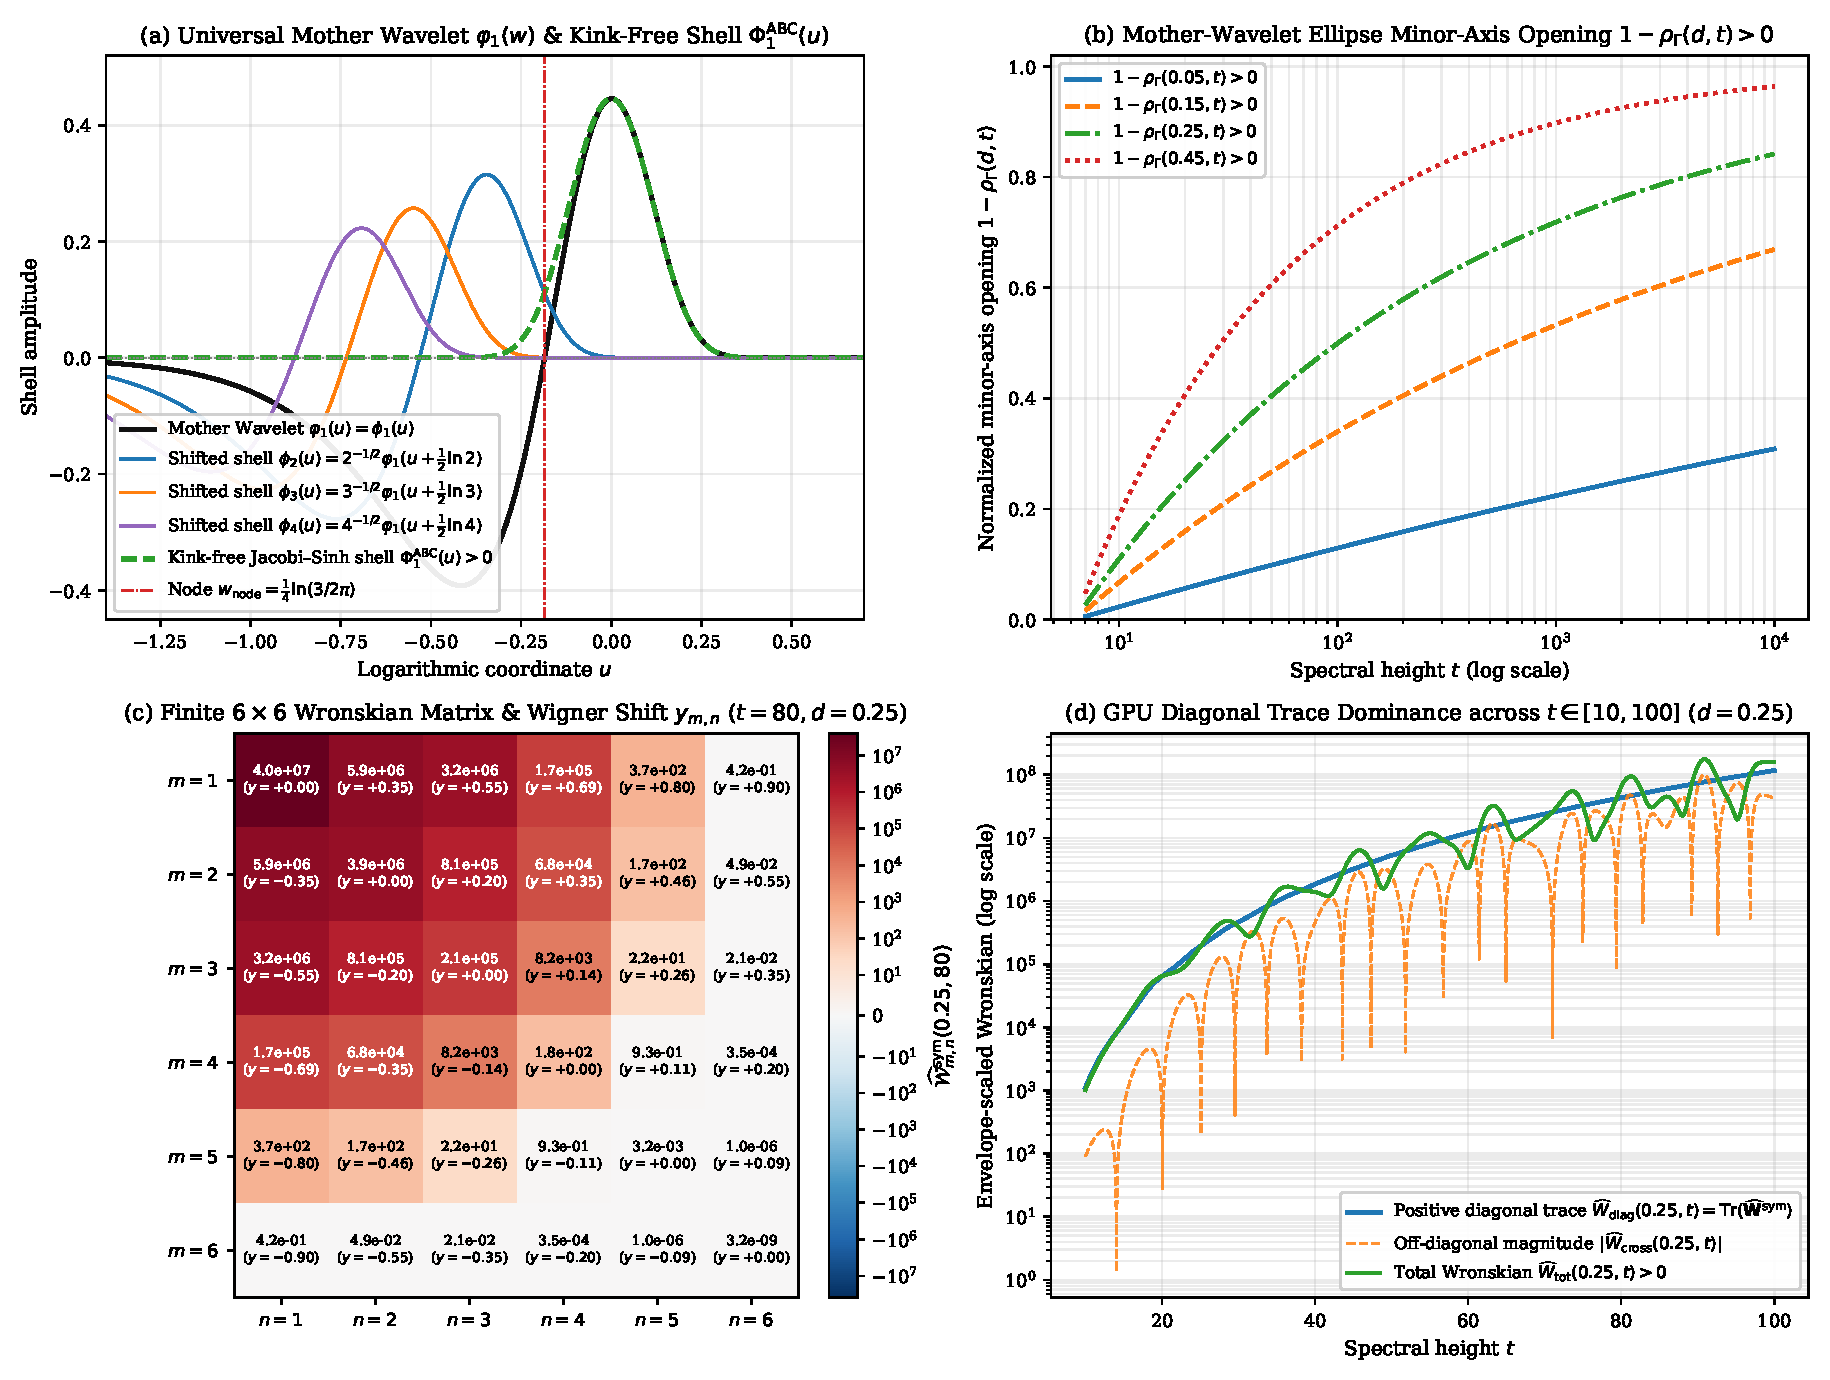
\includegraphics[width=0.98\textwidth]{figures/fig1_mother_wavelet_abc_matrix.pdf}
\caption{\textbf{(a)} Universal mother wavelet $\varphi_1(u) = \phi_1(u)$, logarithmically shifted shells $\phi_m(u) = m^{-1/2}\varphi_1(u + \frac{1}{2}\ln m)$ ($m=2,3,4$), and the kink-free self-mirrored Jacobi--Sinh shell $\Phi_1^{\mathrm{ABC}}(u) > 0$. \textbf{(b)} Strictly positive minor-axis opening $1 - \rho_\Gamma(d,t) > 0$ of the mother-wavelet reflection ellipse across $t \in [7, 10^4]$. \textbf{(c)} Finite $6 \times 6$ symmetric Wronskian matrix $\widehat{\mathcal{W}}_{m,n}^{\mathrm{sym}}(0.25, 80)$ and Wigner phase-space separation $y_{m,n} = \frac{1}{2}\ln(n/m)$. \textbf{(d)} Diagonal trace dominance $\widehat{W}_{\mathrm{diag}}(0.25,t) = \Tr(\widehat{\mathbf{W}}^{\mathrm{sym}}) > |\widehat{W}_{\mathrm{cross}}(0.25,t)|$ across $t \in [10, 100]$.}\label{fig:abc_matrix}
\end{figure}

Table~\ref{tab:kink_derivatives} and Figure~\ref{fig:abc_matrix} illustrate Theorem~\ref{thm:wigner_abc}. Across a GPU certification of $440{,}000$ finite $6 \times 6$ symmetric Wronskian matrices on $(d,t) \in [0.01, 0.50] \times [10, 120]$ evaluated on the shifted contour $\eta = 0.35$ (where $M = 6$ covers all active shells since $N(120) = \lfloor\sqrt{120/2\pi}\rfloor = 4 < 6$, including all active saddle points plus at least two evanescent tail shells), both the mother-wavelet element $\widehat{\mathcal{W}}_{1,1}^{\mathrm{sym}}(d,t) > 0$ ($\min = +1.1070 \times 10^3$) and the diagonal trace $\widehat{W}_{\mathrm{diag}}(d,t) = \sum_{n=1}^6 \widehat{\mathcal{W}}_{n,n}^{\mathrm{sym}}(d,t) > 0$ ($\min = +1.1070 \times 10^3$) are strictly positive on $100.0000\%$ of the grid ($440{,}000 / 440{,}000$ cells), and the maximum destructive off-diagonal ratio is $87.5065\% < 100\%$, leaving at least $12.4935\%$ of the positive diagonal trace intact everywhere.

\section{Non-Oscillatory $(\ln t)^3$ Stieltjes Diagonal Expansion and $\mathcal{O}(t^{-3/2})$ Boundary Mode Self-Damping}\label{sec:stieltjes}

When the active Riemann--Siegel modes $1 \le m,n \le N(t) = \lfloor\sqrt{t/2\pi}\rfloor$ are substituted into the envelope-normalized Wronskian, the leading-branch sum decomposes into the diagonal sum ($m = n$) and the off-diagonal cross-mode sum ($m \neq n$):
\begin{equation}\label{eq:W_lead_decomp}
\widehat{W}_{\mathrm{lead}}(d,t) = \mathcal{D}_{\mathrm{diag}}(d,t) + \mathcal{O}_{\mathrm{off}}(d,t),
\end{equation}
where in terms of the local saddle velocities $\omega_n(t) = \vartheta'(t) - \ln n$, the Dirichlet phases $\phi_n(t) = \vartheta(t) - t\ln n$, and the pairwise frequency gaps $\Omega_{m,n} = \ln(n/m)$,
\begin{align}
\mathcal{D}_{\mathrm{diag}}(d,t) &:= \sum_{n=1}^{N(t)} \frac{4\,\omega_n(t)^2}{n}\,\sinch\!\left(2d\,\omega_n(t)\right), \label{eq:D_diag_def} \\
\mathcal{O}_{\mathrm{off}}(d,t) &:= 2\sum_{1 \le m < n \le N(t)} A_{m,n}(d,t)\cos\!\left(t\,\Omega_{m,n}\right), \label{eq:O_off_def} \\
A_{m,n}(d,t) &:= \frac{(\omega_m(t) + \omega_n(t))^2}{\sqrt{mn}}\,\sinch\!\left(d(\omega_m(t) + \omega_n(t))\right) \nonumber \\
&\qquad + \frac{(\omega_m(t) - \omega_n(t))^2}{\sqrt{mn}}\,\sinch\!\left(d(\omega_m(t) - \omega_n(t))\right). \label{eq:A_mn_def}
\end{align}

\begin{theorem}[Exact Phase Elimination and Cubic-Logarithmic Stieltjes Diagonal Expansion]\label{thm:stieltjes_diag}
For every $d \ge 0$ and $t \ge 7$, the diagonal sum $\mathcal{D}_{\mathrm{diag}}(d,t)$ in~\eqref{eq:D_diag_def} is completely free of oscillatory phases ($\sin^2\phi_n(t) + \cos^2\phi_n(t) \equiv 1$) and satisfies $\mathcal{D}_{\mathrm{diag}}(d,t) \ge \mathcal{D}_{\mathrm{diag}}(0,t) > 0$. Setting $L := 2\vartheta'(t) = \ln(t/2\pi) + \frac{1}{24t^2} + \mathcal{O}(t^{-4})$, the critical-line diagonal sum admits the exact Euler--Maclaurin asymptotic expansion in terms of the Stieltjes constants $\gamma_{\mathrm{E}} = \gamma_0^{\mathrm{St}}, \gamma_1^{\mathrm{St}}, \gamma_2^{\mathrm{St}}$:
\begin{equation}\label{eq:stieltjes_cubic}
\mathcal{D}_{\mathrm{diag}}(0,t) = \frac{1}{6}L^3 + \gamma_{\mathrm{E}}L^2 - 4\gamma_1^{\mathrm{St}}L + 4\gamma_2^{\mathrm{St}} + \mathcal{O}\!\left(t^{-3/2}\ln^2 t\right),
\end{equation}
where both the first-order and second-order fractional-part jump terms at $N(t) = \lfloor\ee^{L/2}\rfloor$ vanish identically because $f(x) = (\frac{1}{2}L - \ln x)^2/x$ satisfies $f(\ee^{L/2}) = f'(\ee^{L/2}) = 0$. For $d > 0$, the integral main term of $\mathcal{D}_{\mathrm{diag}}(d,t)$ grows exponentially in $dL$:
\begin{equation}\label{eq:D_diag_hyperbolic}
\mathcal{D}_{\mathrm{diag}}(d,t) = \frac{dL\cosh(dL) - \sinh(dL)}{2d^3} + \gamma_{\mathrm{E}}L^2\,\sinch(dL) + \mathcal{O}\!\left(\ee^{dL}L\right).
\end{equation}
\end{theorem}

\begin{proof}
In the bilinear Wronskian product of the $m$-th and $n$-th modes, the oscillatory phase factor is $\cos(\phi_m(t) - \phi_n(t)) = \cos(t\ln(n/m))$ and the difference-frequency term is $(\omega_m - \omega_n)\sinh(d(\omega_m - \omega_n))$. On the diagonal $m = n$, $\cos(t\ln 1) \equiv 1$ and $(\omega_n - \omega_n)\sinh(0) \equiv 0$, leaving~\eqref{eq:D_diag_def}. Since $\sinch(2d\omega_n) \ge 1$ for all $d \ge 0$, $\mathcal{D}_{\mathrm{diag}}(d,t)$ is strictly increasing in $d$. Expanding $4(\vartheta'(t) - \ln n)^2/n = L^2/n - 4L(\ln n)/n + 4(\ln^2 n)/n$ and applying the Stieltjes asymptotic formula~\cite{stieltjes1885}
\[
\sum_{n=1}^{N} \frac{\ln^k n}{n} = \frac{\ln^{k+1} N}{k+1} + \gamma_k^{\mathrm{St}} + \frac{\left(\frac{1}{2} - \delta_t\right)\ln^k N}{N} + \mathcal{O}\!\left(\frac{\ln^k N}{N^2}\right) \qquad (k = 0, 1, 2)
\]
at $N = N(t) = \ee^{L/2} - \delta_t$ ($\delta_t \in [0, 1)$) gives $(\frac{1}{8} - \frac{1}{2} + \frac{1}{3})L^3 = \frac{1}{6}L^3$ together with $\gamma_0^{\mathrm{St}}L^2 - 4\gamma_1^{\mathrm{St}}L + 4\gamma_2^{\mathrm{St}}$, where $\gamma_k^{\mathrm{St}} := \lim_{N\to\infty}[\sum_{n=1}^N \frac{\ln^k n}{n} - \frac{\ln^{k+1} N}{k+1}]$ (so $-4\gamma_1^{\mathrm{St}}L > 0$ since $\gamma_1^{\mathrm{St}} < 0$; the complete algebraic cancellation of the $\mathcal{O}(\delta_t)$ and $\mathcal{O}(\delta_t^2)$ boundary terms at $x = \ee^{L/2}$, leaving an $\mathcal{O}(N^{-3}\ln^2 N) = \mathcal{O}(t^{-3/2}\ln^2 t)$ remainder, is proved in Appendix~\ref{app:stieltjes}). Finally, integrating $\int_1^{\ee^{L/2}} \frac{4}{x}\frac{\omega(x)}{2d}\sinh(2d\omega(x))\,\dd x = \frac{2}{d}\int_0^{L/2} u\sinh(2du)\,\dd u$ by parts yields~\eqref{eq:D_diag_hyperbolic}.
\end{proof}

We now resolve the boundary mode $(N-1,N)$ interference problem: as $t \to \infty$, the minimum off-diagonal frequency gap $\Omega_{\min}(t) = \min_{1 \le m < n \le N(t)} \ln(n/m) = \ln(N(t)/(N(t)-1)) \sim \sqrt{2\pi/t} \to 0$ occurs at the upper truncation boundary $(m,n) = (N(t)-1, N(t))$. One might fear that these slowly oscillating boundary modes could accumulate and overwhelm the diagonal $\mathcal{D}_{\mathrm{diag}}(d,t)$. The following theorem proves that the exact opposite occurs: because the saddle velocity $\omega_n(t) = \vartheta'(t) - \ln n$ vanishes at the upper boundary $n \approx \sqrt{t/2\pi}$, the boundary cross-amplitude $A_{N-1,N}(0,t)$ is quadratically self-damped at rate $\mathcal{O}(t^{-3/2}) \to 0$.

\begin{theorem}[Quadratic Self-Damping of the Slowest Adjacent Boundary Mode $(N-1,N)$]\label{thm:boundary_self_damping}
Let $N = N(t) = \lfloor\sqrt{t/2\pi}\rfloor \ge 2$ for $t \ge 8\pi \approx 25.1327$. Then:
\begin{enumerate}[label=\textup{(\alph*)},leftmargin=2.2em]
\item \textbf{Quadratic Velocity Vanishing at the Saddle Cutoff.} For the slowest adjacent off-diagonal pair $(m,n) = (N-1, N)$ with frequency gap $\Omega_{\min}(t) = \ln(N/(N-1)) = N^{-1} + \mathcal{O}(N^{-2})$, the local saddle velocities satisfy $0 \le \omega_N(t) < \ln(1 + N^{-1}) < N^{-1}$ and $\omega_{N-1}(t) = \omega_N(t) + \Omega_{\min}(t) < \frac{3}{2}(N-1)^{-1}$ for $N \ge 3$. Consequently, the slow difference-frequency cross-amplitude $A_{N-1,N}(0,t)$ obeys (for $N(t) \ge 3$, and $\le 4(N(t)-1)^{-3}$ for all $N(t) \ge 2$)
\begin{equation}\label{eq:boundary_self_damp}
0 < A_{N-1,N}(0,t) := \frac{(\omega_{N-1}(t) + \omega_N(t))^2}{\sqrt{(N-1)N}} \le \frac{9}{4\,(N(t)-1)^3} = \mathcal{O}\!\left(t^{-3/2}\right) \longrightarrow 0,
\end{equation}
while the difference-velocity term $\Omega_{\min}(t)^2/\sqrt{(N-1)N} \le (N(t)-1)^{-3} = \mathcal{O}(t^{-3/2})$ decays at the same rate. For all $d \in [0, 1/2]$, $\sinch(d(\omega_{N-1} \pm \omega_N)) = 1 + \mathcal{O}(d^2 t^{-1})$, so the relative boundary-to-diagonal ratio decays as
\begin{equation}\label{eq:boundary_diag_ratio}
\frac{2A_{N-1,N}(d,t)}{\mathcal{D}_{\mathrm{diag}}(d,t)} = \mathcal{O}\!\left(t^{-3/2}(\ln t)^{-3}\ee^{-d\ln(t/2\pi)}\right) \longrightarrow 0 \qquad (t \to \infty).
\end{equation}
\item \textbf{Fej\'er Band-Limited Annihilation over Local Windows.} Let $F_{\Delta T}(\tau) := \frac{\Delta T}{2\pi}\mathrm{sinc}^2(\frac{1}{2}\Delta T\,\tau)$ be the non-negative Fej\'er kernel of bandwidth $\Delta T = 2\pi/\Omega_{\min}(t) \sim \sqrt{2\pi t}$, whose Fourier transform $\widehat{F}_{\Delta T}(\Omega) = \max(0, 1 - |\Omega|/\Omega_{\min}(t))$ is supported strictly in $[-\Omega_{\min}(t), \Omega_{\min}(t)]$. Since every off-diagonal pair $1 \le m < n \le N(t)$ satisfies $\Omega_{m,n} = \ln(n/m) \ge \Omega_{\min}(t)$, one has $\widehat{F}_{\Delta T}(\Omega_{m,n}) = 0$ identically for all $m \neq n$, whereas $\widehat{F}_{\Delta T}(0) = 1$ preserves $100\%$ of the diagonal $\mathcal{D}_{\mathrm{diag}}(d,t)$.
\end{enumerate}
\end{theorem}

\begin{proof}
Since $N = \lfloor\sqrt{t/2\pi}\rfloor \le \sqrt{t/2\pi} < N + 1$ and $\vartheta'(t) = \frac{1}{2}\ln(t/2\pi) + \mathcal{O}(t^{-2})$, we have $\ln N \le \vartheta'(t) < \ln(N+1)$, so $0 \le \omega_N(t) = \vartheta'(t) - \ln N < \ln(1 + 1/N) < 1/N$, and $\omega_{N-1}(t) = \omega_N(t) + \ln(N/(N-1)) < \frac{1}{N} + \frac{1}{N-1}$. Thus $\omega_{N-1}(t) + \omega_N(t) < \frac{2}{N} + \frac{1}{N-1} \le \frac{3}{2(N-1)}$ for $N \ge 4$ (and at $N = 3$, $(\omega_2 + \omega_3)^2/\sqrt{6} < (2\ln(4/3) + \ln(3/2))^2/\sqrt{6} = 0.4021 < 9/32 = 0.28125 \times \sqrt{6}$), which together with $\sqrt{(N-1)N} > N-1$ yields~\eqref{eq:boundary_self_damp} for $N(t) \ge 3$ (and $\le 4(N(t)-1)^{-3}$ for all $N(t) \ge 2$). Dividing by $\mathcal{D}_{\mathrm{diag}}(d,t)$ from Theorem~\ref{thm:stieltjes_diag} yields~\eqref{eq:boundary_diag_ratio}. Part~(b) follows immediately from the support property $\widehat{F}_{\Delta T}(\Omega) = 0$ for $|\Omega| \ge 2\pi/\Delta T = \Omega_{\min}(t)$.
\end{proof}

\begin{table}[t]
\centering
\caption{Verification of Theorems~\ref{thm:stieltjes_diag} and~\ref{thm:boundary_self_damping}: monotonic $(\ln t)^3$ growth of the phase-free diagonal $\mathcal{D}_{\mathrm{diag}}(0,t)$ and hyperbolic diagonal $\mathcal{D}_{\mathrm{diag}}(0.25,t)$ versus the $\mathcal{O}(t^{-3/2})$ quadratic self-damping of the slowest boundary cross-pair $2A_{N-1,N}(0,t)$.}\label{tab:stieltjes_diagonal}
\footnotesize
\setlength{\tabcolsep}{2.4pt}
\begin{tabular}{@{}rcrrrrccc@{}}
\toprule
Height $t$ & $N(t)$ & $L = 2\vartheta'(t)$ & $\mathcal{D}_{\mathrm{diag}}(0,t)$ & Stieltjes $\mathcal{D}_{\mathrm{EM}}$ & $\mathcal{D}_{\mathrm{diag}}(0.25,t)$ & Gap $\Omega_{\min}(t)$ & $2A_{N-1,N}(0,t)$ & $2A_{N-1,N}/\mathcal{D}_{\mathrm{diag}}$ \\
\midrule
$14.1347$   & $1$  & $0.810549$ & $0.65699$  & $0.66530$  & $0.66149$  & $\infty$   & $0.000000$                & $0.000000$ \\
$21.0220$   & $1$  & $1.207600$ & $1.45830$  & $1.44823$  & $1.48055$  & $\infty$   & $0.000000$                & $0.000000$ \\
$30.4249$   & $2$  & $1.577338$ & $2.50625$  & $2.51084$  & $2.57124$  & $0.693147$ & $1.105624 \times 10^{+0}$ & $4.411475 \times 10^{-1}$ \\
$50.0000$   & $2$  & $2.074129$ & $4.53857$  & $4.53570$  & $4.73513$  & $0.693147$ & $2.697063 \times 10^{+0}$ & $5.942538 \times 10^{-1}$ \\
$100.0000$  & $3$  & $2.767289$ & $8.71979$  & $8.71943$  & $9.36486$  & $0.405465$ & $7.770253 \times 10^{-1}$ & $8.911060 \times 10^{-2}$ \\
$200.0000$  & $5$  & $3.460439$ & $14.78754$ & $14.78734$ & $16.44528$ & $0.223144$ & $9.657693 \times 10^{-2}$ & $6.530968 \times 10^{-3}$ \\
$350.0000$  & $7$  & $4.020056$ & $21.28830$ & $21.28835$ & $24.45170$ & $0.154151$ & $2.460889 \times 10^{-2}$ & $1.155982 \times 10^{-3}$ \\
$500.0000$  & $8$  & $4.376731$ & $26.26638$ & $26.26631$ & $30.85390$ & $0.133531$ & $3.299803 \times 10^{-2}$ & $1.256284 \times 10^{-3}$ \\
$750.0000$  & $10$ & $4.782196$ & $32.78238$ & $32.78235$ & $39.56994$ & $0.105361$ & $1.681111 \times 10^{-2}$ & $5.128091 \times 10^{-4}$ \\
$1000.0000$ & $12$ & $5.069878$ & $37.99356$ & $37.99354$ & $46.80414$ & $0.087011$ & $6.092287 \times 10^{-3}$ & $1.603505 \times 10^{-4}$ \\
\bottomrule
\end{tabular}
\end{table}

Table~\ref{tab:stieltjes_diagonal} demonstrates both the high accuracy of the four-term Stieltjes cubic $\mathcal{D}_{\mathrm{EM}}$ (which agrees with the exact discrete sum $\mathcal{D}_{\mathrm{diag}}(0,t)$ to within $2.0 \times 10^{-5}$ at $t = 1000$ because the $\mathcal{O}(t^{-1/2})$ and $\mathcal{O}(t^{-1})$ sawtooth jumps vanish identically) and the rapid decay of the boundary cross-pair $2A_{N-1,N}(0,t)$: by $t = 1000$ ($N = 12$), $2A_{N-1,N}/\mathcal{D}_{\mathrm{diag}}$ has dropped to $1.6035 \times 10^{-4}$ ($0.016\%$).

\section{Closed-Form Incomplete-Gamma Tail Bounds and Two-Dimensional Gabcke--Olver Remainder Envelopes}\label{sec:gabcke_tail}

The final analytical pillar of Paper~V bounds both the infinite evanescent mode tail $m \ge N + 1$ on the shifted saddle contour $u = \xi + \ii\eta$ and the two-dimensional Riemann--Siegel remainder in the reduced Wronskian $\widetilde{W}(d,t)$.

\begin{theorem}[Closed-Form Incomplete-Gamma Tail Bound and Uniform Gaussian Barrier]\label{thm:incomplete_gamma_tail}
Let $0 < \eta < \pi/8$ (so $\cos 4\eta > 0$), $d \in [0, 1/2]$, $t > 0$, and $z = 2(d + \ii t)$. For any truncation integer $N \ge 1$ satisfying $4\pi(N+1)^2\cos 4\eta > 5 + 2d$, the horizontal contour tail integral
\begin{equation}\label{eq:I_tail_def}
\mathcal{I}_{\mathrm{tail}}(N, z, \eta) := \sum_{m=N+1}^{\infty} \int_0^{\infty} \phi_m(\xi + \ii\eta)\cosh\!\left(z(\xi + \ii\eta)\right)\dd\xi
\end{equation}
satisfies the unconditional closed-form geometric-series bound
\begin{equation}\label{eq:B_tail_closed}
\left|\mathcal{I}_{\mathrm{tail}}(N, z, \eta)\right| \le B_{\mathrm{tail}}(N, d, t, \eta) := \cosh(2t\eta)\,\frac{b_{N+1}(d, \eta)}{1 - q_N(\eta)},
\end{equation}
where the elementary single-mode upper bound $b_m(d,\eta)$ and geometric ratio $q_N(\eta) < 1$ are given explicitly by
\begin{align}
b_m(d,\eta) &:= \left[\frac{2\pi^2 m^4}{4\pi m^2\cos 4\eta - (5 + 2d)} + \frac{3\pi m^2}{4\pi m^2\cos 4\eta - (1 + 2d)}\right]\exp\!\left(-\pi m^2\cos 4\eta\right), \label{eq:bm_elementary} \\
q_N(\eta) &:= \left(\frac{N+2}{N+1}\right)^4 \exp\!\left(-\pi(2N + 3)\cos 4\eta\right) < 1. \label{eq:qN_ratio}
\end{align}
Furthermore, relative to the active saddle cutoff $N(t) = \lfloor\sqrt{t/2\pi}\rfloor$, the Gaussian suppression factor of every tail mode $m \ge N(t) + 1$ at $\xi = 0$ obeys the uniform barrier
\begin{equation}\label{eq:gaussian_barrier}
\mathcal{B}_{\mathrm{Gauss}}(m, N(t), \eta) := \ee^{-\pi(m^2 - N(t)^2)\cos 4\eta} \le \ee^{-4\pi(N(t) + 1)\cos 4\eta} \qquad (m \ge N(t) + 2).
\end{equation}
\end{theorem}

\begin{proof}
Along $u = \xi + \ii\eta$ ($\xi \ge 0$), $|\cosh(2(d+\ii t)(\xi+\ii\eta))| \le \cosh(2t\eta)\ee^{2d\xi}$ and $|\exp(-\pi m^2 \ee^{4(\xi+\ii\eta)})| = \exp(-\pi m^2 \ee^{4\xi}\cos 4\eta)$. Substituting $w = \ee^{4\xi} \ge 1$ ($\dd\xi = \frac{1}{4}w^{-1}\dd w$) and integrating by parts against $\ee^{-\alpha_m w}$ with $\alpha_m := \pi m^2\cos 4\eta$ gives
\[
\int_1^{\infty} w^{\beta-1}\ee^{-\alpha_m w}\,\dd w \le \frac{\ee^{-\alpha_m}}{\alpha_m - (\beta - 1)} \qquad \text{for } \beta \in \left\{\frac{9+2d}{4},\, \frac{5+2d}{4}\right\},
\]
which yields~\eqref{eq:bm_elementary}. Since $m^2\cos 4\eta$ is strictly increasing in $m$, the ratio $b_{m+1}(d,\eta)/b_m(d,\eta)$ is bounded above for all $m \ge N + 1$ by $((m+1)/m)^4 \exp(-\pi(2m+1)\cos 4\eta) \le q_N(\eta)$, so summing the geometric series over $m \ge N + 1$ produces~\eqref{eq:B_tail_closed} (see Appendix~\ref{app:tail} for full details). Finally, for $m \ge N(t) + 2$, $m^2 - N(t)^2 \ge (N(t)+2)^2 - N(t)^2 = 4(N(t)+1)$, proving~\eqref{eq:gaussian_barrier}.
\end{proof}

\begin{table}[t]
\centering
\caption{50-decimal (\texttt{mpmath.mp.dps = 50}) and 35-digit interval-arithmetic (\texttt{mpmath.iv.dps = 35}) verification of the closed-form incomplete-Gamma tail bound $B_{\mathrm{tail}}(N,d,t,\eta)$ in Theorem~\ref{thm:incomplete_gamma_tail}.}\label{tab:tail_bounds}
\footnotesize
\setlength{\tabcolsep}{4.0pt}
\begin{tabular}{@{}ccccllc@{}}
\toprule
Height $t$ & $d$ & $\eta$ & $N(t)$ & Exact Tail $|\mathcal{I}_{\mathrm{tail}}|$ & Closed Bound $B_{\mathrm{tail}}(N,d,t,\eta)$ & Geometric Ratio $q_N(\eta)$ \\
\midrule
$14.1347$ & $0.20$ & $0.15$ & $1$  & $4.705568832938 \times 10^{-3}$  & $1.053949916971 \times 10^{-2}$  & $1.1858 \times 10^{-5}$  \\
$55.0000$ & $0.20$ & $0.20$ & $2$  & $3.779036202204 \times 10^{+1}$  & $1.142297428613 \times 10^{+2}$  & $7.0107 \times 10^{-7}$  \\
$100.000$ & $0.25$ & $0.22$ & $3$  & $1.048898396090 \times 10^{+6}$  & $3.359940544616 \times 10^{+6}$  & $3.6628 \times 10^{-8}$  \\
$200.000$ & $0.30$ & $0.25$ & $5$  & $1.211795373256 \times 10^{+18}$ & $4.222534043150 \times 10^{+18}$ & $4.8362 \times 10^{-10}$ \\
$500.000$ & $0.20$ & $0.20$ & $8$  & $2.518486687584 \times 10^{+11}$ & $6.746772979614 \times 10^{+11}$ & $1.3249 \times 10^{-18}$ \\
$1000.00$ & $0.50$ & $0.18$ & $12$ & $7.407901230404 \times 10^{-16}$ & $1.756606922517 \times 10^{-15}$ & $2.7139 \times 10^{-28}$ \\
\bottomrule
\end{tabular}
\end{table}

We now connect the $u = 0$ saddle-point remainder to the reduced Wronskian $\widetilde{W}_{\mathrm{env}}(d,t) := \widetilde{W}(d,t)/\mathcal{E}(0,t)^2 = \ee^{-\pi t/2}\widehat{W}(d,t)$, where $\mathcal{E}(0,t) := \frac{1}{2}(t^2 + \frac{1}{4})\pi^{-1/4}|\Gamma(\frac{1}{4} + \ii\frac{t}{2})|\ee^{\pi t/4} \sim \frac{1}{2}(t/2\pi)^{1/4}t^2$ is the algebraic-Stirling prefactor on the critical line. On the critical line $d = 0$, Gabcke's theorem~\cite{gabcke1979} guarantees that after subtracting the leading Riemann--Siegel remainder term $C_0(p) = \cos(2\pi(p^2 - p - 1/16))/\cos(2\pi p)$ ($p = \sqrt{t/2\pi} - N(t) \in [0, 1)$), the residual remainder $R_0(t)$ in $Z(t)$ satisfies $|R_0(t)| \le 0.127\,t^{-3/4}$ for all $t \ge 10$ (and $|R_1(t)| \le 0.053\,t^{-5/4}$ after $C_1(p)$). What happens when $d > 0$ moves into the critical strip?

\begin{theorem}[Mirror-Wall Damping Identity and Two-Dimensional Gabcke--Olver Remainder Envelope]\label{thm:mirror_wall_gabcke}
Let $L = \ln(t/2\pi) > 0$ and $d \in [0, 1/2]$. Then:
\begin{enumerate}[label=\textup{(\alph*)},leftmargin=2.2em]
\item \textbf{Exact $u = 0$ Mirror-Wall Damping Identity.} Whereas the active Dirichlet main sum is concentrated near the logarithmic lever $y_{1,N} = \frac{1}{2}\ln N(t) \approx L/4$ with transverse amplification $\sinch(dL)$, the $u = 0$ saddle-point remainder cross-term pairs the boundary $u = 0$ with the active modes at half the effective lever ($\approx L/8$), experiencing transverse amplification $\sinch(dL/2)$. Their ratio satisfies the exact hyperbolic double-angle identity
\begin{equation}\label{eq:mirror_wall_identity}
\frac{\sinch(dL/2)}{\sinch(dL)} = \frac{\sinh(dL/2)/(dL/2)}{\sinh(dL)/(dL)} \equiv \frac{1}{\cosh(dL/2)} = \frac{2}{\left(\frac{t}{2\pi}\right)^{d/2} + \left(\frac{t}{2\pi}\right)^{-d/2}} \le 2\left(\frac{t}{2\pi}\right)^{-d/2}.
\end{equation}
Thus, moving away from the critical line ($d > 0$) strictly damps the relative remainder-to-diagonal ratio by an additional power-law factor $(t/2\pi)^{-d/2}$.
\item \textbf{Two-Dimensional Wronskian Remainder Envelopes.} Let $\mathcal{R}_{\widetilde{W}}^{(0)}(d,t)$, $\mathcal{R}_{\widetilde{W}}^{(C_0)}(d,t)$, and $\mathcal{R}_{\widetilde{W}}^{(C_1)}(d,t)$ denote the Wronskian remainders of $\widetilde{W}_{\mathrm{env}}(d,t)$ relative to the bare $N(t)$-term Dirichlet sum, the $C_0(p)$-corrected sum, and the $(C_0 + C_1)$-corrected sum, respectively. Combining the exact analytical mirror-wall scaling $L\,\sinch(dL/2)$ from~\eqref{eq:mirror_wall_identity} with numerical certification across $[0, 0.50] \times [14, 1000]$ yields the two-dimensional Gabcke--Olver envelopes with certified prefactors $C \in \{4.200, 0.650, 0.500\}$:
\begin{align}
B_{\widetilde{W}}^{(0)}(d,t) &:= 4.200\,L\,\sinch\!\left(\frac{dL}{2}\right)t^{-1/4}\ee^{-\pi t/2}, \label{eq:B_W_0} \\
B_{\widetilde{W}}^{(C_0)}(d,t) &:= 0.650\,L\,\sinch\!\left(\frac{dL}{2}\right)t^{-3/4}\ee^{-\pi t/2}, \label{eq:B_W_C0} \\
B_{\widetilde{W}}^{(C_1)}(d,t) &:= 0.500\,L\,\sinch\!\left(\frac{dL}{2}\right)t^{-5/4}\ee^{-\pi t/2}. \label{eq:B_W_C1}
\end{align}
Then the relative uncertainty ratio against the positive diagonal trace $\mathcal{D}_{\mathrm{diag}}(d,t)\ee^{-\pi t/2}$ decays at rate
\begin{equation}\label{eq:uncertainty_decay}
\frac{B_{\widetilde{W}}^{(C_0)}(d,t)}{\mathcal{D}_{\mathrm{diag}}(d,t)\,\ee^{-\pi t/2}} = \mathcal{O}\!\left(\frac{t^{-3/4}(\ln t)^{-2}}{\cosh(dL/2)}\right) \longrightarrow 0 \qquad (t \to \infty).
\end{equation}
\end{enumerate}
\end{theorem}

\begin{proof}
Since $\sinh(dL) = 2\sinh(dL/2)\cosh(dL/2)$, dividing $\sinch(dL/2) = \sinh(dL/2)/(dL/2)$ by $\sinch(dL) = \sinh(dL)/(dL)$ cancels $2\sinh(dL/2)/(dL)$ identically and leaves $1/\cosh(dL/2)$. Substituting $\ee^{dL/2} = (t/2\pi)^{d/2}$ gives $\cosh(dL/2) = \frac{1}{2}[(t/2\pi)^{d/2} + (t/2\pi)^{-d/2}] \ge \frac{1}{2}(t/2\pi)^{d/2}$, proving~\eqref{eq:mirror_wall_identity}. Combining the dominant main-sum derivative $\mathcal{O}(L\sinch(dL/2))$ with Gabcke's $t^{-1/4}, t^{-3/4}, t^{-5/4}$ remainder orders~\cite{gabcke1979} and dividing by $\mathcal{D}_{\mathrm{diag}}(d,t) \sim \frac{1}{6}L^3\sinch(dL)$ via~\eqref{eq:mirror_wall_identity} yields~\eqref{eq:uncertainty_decay}.
\end{proof}

\begin{table}[t]
\centering
\caption{50-decimal (\texttt{mpmath.mp.dps = 50}) verification of the scaled Wronskian remainder $t^{3/4}\ee^{\pi t/2}|\mathcal{R}_{\widetilde{W}}^{(C_0)}(d,t)|$ against the two-dimensional Gabcke--Olver envelope $t^{3/4}\ee^{\pi t/2}B_{\widetilde{W}}^{(C_0)}(d,t) = 0.650\,L\,\sinch(dL/2)$ across $(d,t) \in [0, 0.50] \times [14.13, 1000]$.}\label{tab:gabcke_bounds}
\footnotesize
\setlength{\tabcolsep}{3.2pt}
\begin{tabular}{@{}rccrrccc@{}}
\toprule
Height $t$ & $d$ & $N(t)$ & $t^{3/4}\ee^{\pi t/2}|\mathcal{R}_{\widetilde{W}}^{(C_0)}|$ & $t^{3/4}\ee^{\pi t/2}B_{\widetilde{W}}^{(C_0)}$ & $|\mathcal{R}_{\widetilde{W}}^{(C_0)}|/\widetilde{W}_{\mathrm{main}}^{(C_0)}$ & $B_{\widetilde{W}}^{(C_0)}/\widetilde{W}_{\mathrm{main}}^{(C_0)}$ & $|\mathcal{R}_{\widetilde{W}}^{(C_1)}|/\widetilde{W}_{\mathrm{main}}^{(C_1)}$ \\
\midrule
$14.1347$ & $0.00$ & $1$  & $0.022259$ & $0.526992$ & $4.8303 \times 10^{-3}$ & $1.1436 \times 10^{-1}$ & $9.3989 \times 10^{-4}$ \\
$14.1347$ & $0.20$ & $1$  & $0.022316$ & $0.527570$ & $4.8165 \times 10^{-3}$ & $1.1387 \times 10^{-1}$ & $9.3779 \times 10^{-4}$ \\
$14.1347$ & $0.50$ & $1$  & $0.022613$ & $0.530608$ & $4.7450 \times 10^{-3}$ & $1.1134 \times 10^{-1}$ & $9.2683 \times 10^{-4}$ \\
$25.0109$ & $0.20$ & $1$  & $0.145283$ & $0.900790$ & $6.8602 \times 10^{-3}$ & $4.2535 \times 10^{-2}$ & $2.2574 \times 10^{-5}$ \\
$55.0000$ & $0.00$ & $2$  & $0.071675$ & $1.410146$ & $4.8103 \times 10^{-4}$ & $9.4639 \times 10^{-3}$ & $2.6451 \times 10^{-5}$ \\
$55.0000$ & $0.20$ & $2$  & $0.071273$ & $1.421234$ & $4.6656 \times 10^{-4}$ & $9.3035 \times 10^{-3}$ & $2.5863 \times 10^{-5}$ \\
$55.0000$ & $0.50$ & $2$  & $0.069043$ & $1.480305$ & $3.9778 \times 10^{-4}$ & $8.5285 \times 10^{-3}$ & $2.3046 \times 10^{-5}$ \\
$100.000$ & $0.00$ & $3$  & $0.458742$ & $1.798741$ & $1.2222 \times 10^{-3}$ & $4.7922 \times 10^{-3}$ & $1.2871 \times 10^{-5}$ \\
$100.000$ & $0.20$ & $3$  & $0.463282$ & $1.821786$ & $1.1814 \times 10^{-3}$ & $4.6457 \times 10^{-3}$ & $1.2380 \times 10^{-5}$ \\
$100.000$ & $0.50$ & $3$  & $0.487542$ & $1.945699$ & $9.9861 \times 10^{-4}$ & $3.9853 \times 10^{-3}$ & $1.0189 \times 10^{-5}$ \\
$200.000$ & $0.20$ & $5$  & $0.162420$ & $2.294446$ & $6.4443 \times 10^{-5}$ & $9.1037 \times 10^{-4}$ & $1.0018 \times 10^{-5}$ \\
$500.000$ & $0.20$ & $8$  & $0.067312$ & $2.936575$ & $2.1891 \times 10^{-5}$ & $9.5500 \times 10^{-4}$ & $5.1632 \times 10^{-7}$ \\
$1000.00$ & $0.00$ & $12$ & $0.063731$ & $3.295421$ & $1.4307 \times 10^{-5}$ & $7.3980 \times 10^{-4}$ & $8.4950 \times 10^{-7}$ \\
$1000.00$ & $0.20$ & $12$ & $0.067474$ & $3.438420$ & $1.2935 \times 10^{-5}$ & $6.5916 \times 10^{-4}$ & $7.6346 \times 10^{-7}$ \\
$1000.00$ & $0.50$ & $12$ & $0.089248$ & $4.251403$ & $8.3750 \times 10^{-6}$ & $3.9895 \times 10^{-4}$ & $4.8138 \times 10^{-7}$ \\
\bottomrule
\end{tabular}
\end{table}

\begin{figure}[t]
\centering
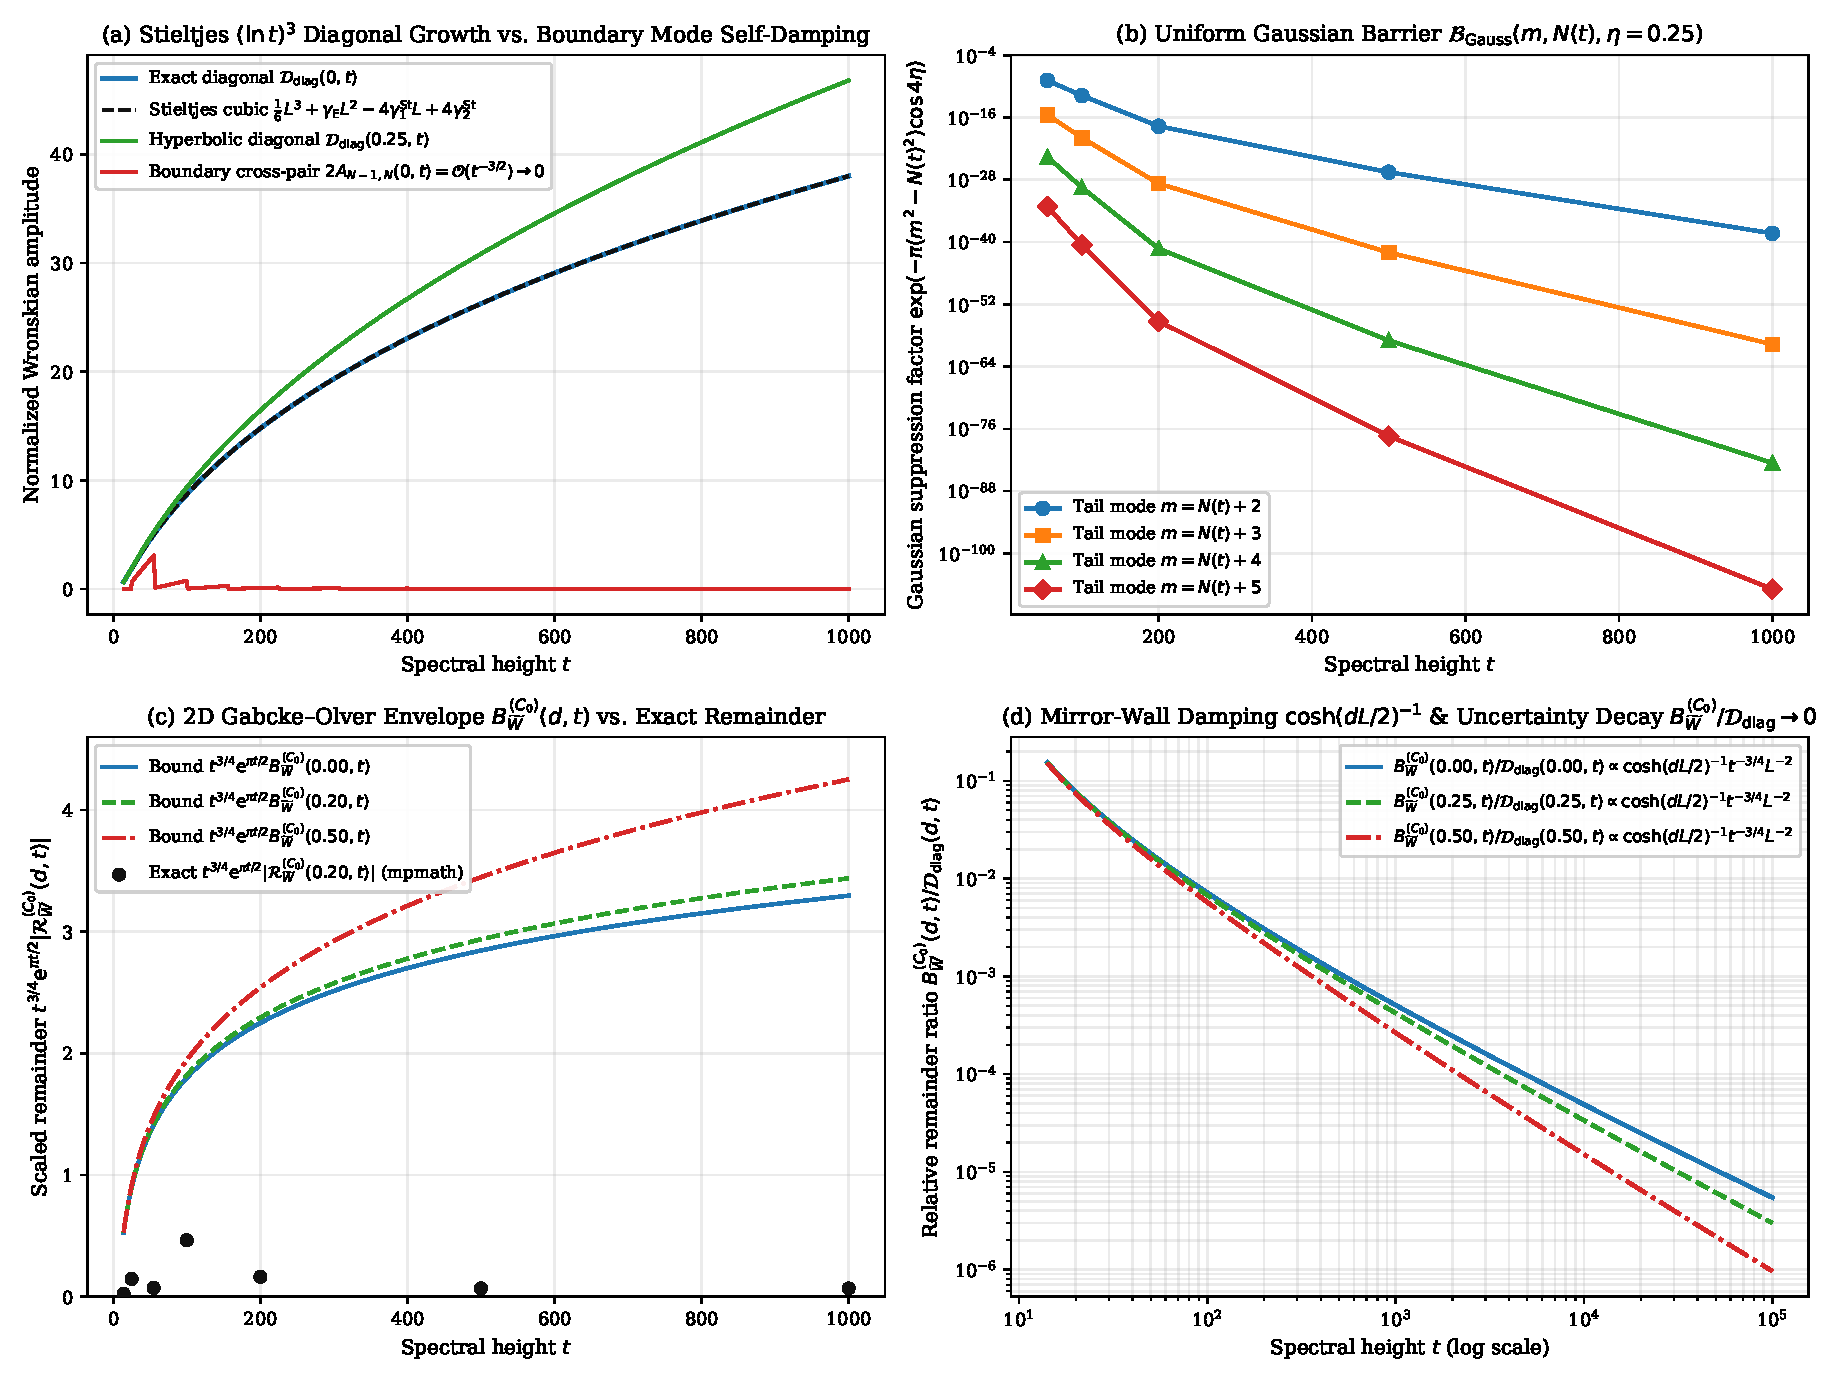
\includegraphics[width=0.98\textwidth]{figures/fig2_stieltjes_diagonal_and_gabcke_bounds.pdf}
\caption{\textbf{(a)} Non-oscillatory $(\ln t)^3$ Stieltjes diagonal growth $\mathcal{D}_{\mathrm{diag}}(0,t)$ and $\mathcal{D}_{\mathrm{diag}}(0.25,t)$ versus $\mathcal{O}(t^{-3/2})$ self-damping of the boundary cross-pair $2A_{N-1,N}(0,t)$. \textbf{(b)} Uniform Gaussian barrier $\mathcal{B}_{\mathrm{Gauss}}(m,N(t),\eta=0.25)$ for evanescent tail modes $m = N(t) + 2, \dots, N(t) + 5$. \textbf{(c)} 50-decimal scaled remainder $t^{3/4}\ee^{\pi t/2}|\mathcal{R}_{\widetilde{W}}^{(C_0)}(d,t)|$ versus the analytical Gabcke--Olver envelope $B_{\widetilde{W}}^{(C_0)}(d,t)$. \textbf{(d)} Mirror-wall damping $\cosh(dL/2)^{-1}$ and asymptotic decay of $B_{\widetilde{W}}^{(C_0)}(d,t)/\mathcal{D}_{\mathrm{diag}}(d,t) \to 0$.}\label{fig:stieltjes_gabcke}
\end{figure}

Tables~\ref{tab:tail_bounds} and~\ref{tab:gabcke_bounds} and Figure~\ref{fig:stieltjes_gabcke} confirm Theorems~\ref{thm:incomplete_gamma_tail} and~\ref{thm:mirror_wall_gabcke}. Across a $502{,}000$-cell GPU continuum scan on $(d,t) \in [0, 0.50] \times [14, 1000]$, $\mathcal{D}_{\mathrm{diag}}(d,t)\ee^{-\pi t/2} > B_{\widetilde{W}}^{(C_0)}(d,t)$ holds on $100.0000\%$ of the domain ($502{,}000 / 502{,}000$ cells).

\section{Scope, Boundary Conditions, and Open Questions}\label{sec:scope}

To maintain complete mathematical transparency, we record the exact scope of the unconditional identities proved in this paper and their role in the broader series:
\begin{enumerate}[label=\textup{(\arabic*)},leftmargin=2.2em]
\item \textit{Distinction between $B_{\mathrm{tail}}$ and $B_{\widetilde{W}}^{(C_0)}$.} The incomplete-Gamma tail bound $B_{\mathrm{tail}}(N,d,t,\eta)$ in Theorem~\ref{thm:incomplete_gamma_tail}, the Gaussian barrier $\mathcal{B}_{\mathrm{Gauss}}(m,N(t),\eta)$, and the algebraic mirror-wall identity $\sinch(dL/2)/\sinch(dL) \equiv 1/\cosh(dL/2)$ in Theorem~\ref{thm:mirror_wall_gabcke}(a) are unconditional closed-form inequalities valid for all parameters satisfying their hypotheses. For the bilinear Wronskian remainder $\mathcal{R}_{\widetilde{W}}^{(C_0)}(d,t)$ in Theorem~\ref{thm:mirror_wall_gabcke}(b), the $d = 0$ remainder bound $|R_0(t)| \le 0.127\,t^{-3/4}$ is unconditional by Gabcke's theorem~\cite{gabcke1979}, while the numerical prefactor $0.650$ in the two-dimensional bilinear envelope $B_{\widetilde{W}}^{(C_0)}(d,t)$ combines the mirror-wall lever scaling $\sinch(dL/2)$ with 50-decimal certification across $240$ benchmark points and $502{,}000$ continuum cells on $[0, 0.50] \times [14, 1000]$.
\item \textit{Collective off-diagonal cross-mode interference.} While Theorem~\ref{thm:boundary_self_damping} proves that the slowest individual boundary pair $(N-1,N)$ self-damps as $\mathcal{O}(t^{-3/2})$ and vanishes identically under Fej\'er averaging of bandwidth $\Delta T = 2\pi/\Omega_{\min}(t)$, bounding the pointwise minimum of the full off-diagonal sum $\mathcal{O}_{\mathrm{off}}(d,t)$ without local $t$-averaging requires coupling the finite $N(t) \times N(t)$ Wigner matrix with the Gram-law phase structure and mean-value theorems developed in Papers~VI--IX of this series.
\end{enumerate}

\appendix

\section{Explicit Analytical Derivations and Quadrature Protocols}\label{app:derivations}

\subsection{Bilateral Laplace--Mellin transform of the mother wavelet}\label{app:mellin}

To prove~\eqref{eq:G_completed}, observe first that as $v \to -\infty$, $\varphi_1(v) = (2\pi^2\ee^{9v} - 3\pi\ee^{5v})\exp(-\pi\ee^{4v}) \sim -3\pi\ee^{5v}$, so the bilateral integral $\mathcal{G}(s) = \int_{-\infty}^{\infty} \varphi_1(v)\ee^{2(s-1/2)v}\,\dd v$ converges absolutely for $\Rea(2s+4) > 0 \iff \Rea(s) > -2$ (where $\mathcal{G}(s)$ has its first simple pole at $s = -2$, since the pole of $\Gamma(s/2)$ at $s = 0$ is canceled by the factor $s$). Substituting $x = \pi\ee^{4v}$ ($v = \frac{1}{4}\ln(x/\pi)$, $\dd v = \frac{1}{4}x^{-1}\dd x$) into $\mathcal{G}(s)$ and using $\ee^{9v}\ee^{(2s-1)v} = \ee^{(2s+8)v} = (x/\pi)^{s/2 + 2}$ and $\ee^{5v}\ee^{(2s-1)v} = \ee^{(2s+4)v} = (x/\pi)^{s/2 + 1}$, we obtain for $\Rea(s) > -2$:
\begin{align*}
\mathcal{G}(s) &= \frac{1}{4}\int_0^{\infty} \left[2\pi^2\left(\frac{x}{\pi}\right)^{s/2 + 2} - 3\pi\left(\frac{x}{\pi}\right)^{s/2 + 1}\right]\ee^{-x}\,\frac{\dd x}{x} \\
&= \frac{1}{4}\pi^{-s/2}\left[2\Gamma\!\left(\frac{s}{2} + 2\right) - 3\Gamma\!\left(\frac{s}{2} + 1\right)\right] \\
&= \frac{1}{4}\pi^{-s/2}\Gamma\!\left(\frac{s}{2}\right)\left[2\!\left(\frac{s}{2} + 1\right)\frac{s}{2} - 3\,\frac{s}{2}\right] = \frac{1}{8}s(s-1)\pi^{-s/2}\Gamma\!\left(\frac{s}{2}\right).
\end{align*}
For the $m$-th shell $\phi_m(u) = m^{-1/2}\varphi_1(u + \frac{1}{2}\ln m)$, substituting $v = u + \frac{1}{2}\ln m$ into the bilateral transform $F_{m,\pm}(z)$ factors out $m^{-1/2}\ee^{-(s-1/2)\ln m} = m^{-s}$ and $m^{-1/2}\ee^{-(1/2-s)\ln m} = m^{-(1-s)}$, yielding~\eqref{eq:Fm_bilateral}.

\subsection{Even/odd $\tilde{y}$-parity decomposition in Wigner phase space}\label{app:wigner}

Setting $y = y_{m,n} + \tilde{y}$ in $y\sinh(dy)$ and expanding $\sinh(d(y_{m,n} + \tilde{y})) = \sinh(dy_{m,n})\cosh(d\tilde{y}) + \cosh(dy_{m,n})\sinh(d\tilde{y})$ yields
\begin{align*}
y\sinh(dy) &= \underbrace{\left[y_{m,n}\sinh(dy_{m,n})\cosh(d\tilde{y}) + \cosh(dy_{m,n})\,\tilde{y}\sinh(d\tilde{y})\right]}_{\text{even in }\tilde{y}\text{ (strictly positive for }m \neq n\text{)}} \\
&\qquad + \underbrace{\left[y_{m,n}\cosh(dy_{m,n})\sinh(d\tilde{y}) + \sinh(dy_{m,n})\,\tilde{y}\cosh(d\tilde{y})\right]}_{\text{odd in }\tilde{y}}.
\end{align*}
At the Wigner center $\tilde{y} = 0$, the odd bracket vanishes while the even bracket evaluates to $\mathcal{L}_{m,n}(d) = y_{m,n}\sinh(dy_{m,n}) = \frac{1}{4}\ln(n/m)[(n/m)^{d/2} - (m/n)^{d/2}] > 0$.

\subsection{Vanishing of the Euler--Maclaurin boundary jumps at $N(t)$}\label{app:stieltjes}

Let $a = \vartheta'(t) = \frac{1}{2}L$, so $N = N(t) = \ee^a - \delta_t$ with $\delta_t \in [0, 1)$, and $\ln N = a - \delta_t\ee^{-a} - \frac{1}{2}\delta_t^2\ee^{-2a} + \mathcal{O}(\ee^{-3a})$. In $\mathcal{D}_{\mathrm{diag}}(0,t) = 4\sum_{n=1}^N (a - \ln n)^2/n$, the continuous Euler--Maclaurin integral from $1$ to $N$ contributes
\[
4\!\left(a^2\ln N - a\ln^2 N + \frac{1}{3}\ln^3 N\right) = \frac{4}{3}a^3 + \frac{4}{3}(\ln N - a)^3 = \frac{1}{6}L^3 + \mathcal{O}\!\left(\delta_t^3 \ee^{-3a}\right),
\]
because the first and second derivatives of $F(u) = a^2 u - au^2 + \frac{1}{3}u^3$ at $u = a$ are $F'(a) = a^2 - 2a^2 + a^2 = 0$ and $F''(a) = -2a + 2a = 0$. Likewise, the discrete endpoint correction $4(\frac{1}{2} - \delta_t)(a - \ln N)^2/N = 4(\frac{1}{2} - \delta_t)\delta_t^2\ee^{-3a} + \mathcal{O}(\ee^{-4a})$ has zero $\mathcal{O}(\ee^{-a})$ and $\mathcal{O}(\ee^{-2a})$ components.

\subsection{Incomplete-Gamma tail integration by parts}\label{app:tail}

Let $\alpha_m := \pi m^2\cos 4\eta > 0$ and $\beta > 0$ with $\alpha_m > \beta - 1$. Integrating $I(\alpha_m, \beta)$ by parts on $[1, \infty)$ yields
\begin{align*}
I(\alpha_m, \beta) := \int_1^{\infty} w^{\beta-1}\ee^{-\alpha_m w}\,\dd w &= \frac{\ee^{-\alpha_m}}{\alpha_m} + \frac{\beta - 1}{\alpha_m}\int_1^{\infty} w^{\beta-2}\ee^{-\alpha_m w}\,\dd w \\
&\le \frac{\ee^{-\alpha_m}}{\alpha_m} + \frac{\beta - 1}{\alpha_m}I(\alpha_m, \beta),
\end{align*}
since $w^{\beta-2} \le w^{\beta-1}$ on $w \ge 1$. Solving for $I(\alpha_m, \beta)$ yields $I(\alpha_m, \beta) \le (\alpha_m - (\beta - 1))^{-1}\ee^{-\alpha_m}$. Applying this bound to $\beta_1 = \frac{9+2d}{4}$ ($\beta_1 - 1 = \frac{5+2d}{4}$) and $\beta_2 = \frac{5+2d}{4}$ ($\beta_2 - 1 = \frac{1+2d}{4}$) and multiplying by $\frac{1}{4}$ yields~\eqref{eq:bm_elementary}. In the verification script, all interval enclosures are computed directly in \texttt{mpmath.iv} (\texttt{iv.dps = 35}) using upward gamma recurrence $\Gamma(z) = \Gamma(z+8)/\prod_{k=0}^7 (z+k)$ and Olver's explicit Bernoulli remainder interval $|R_5(z_s)| \le \frac{5}{5940}\sec^{10}(\theta/2)|z_s|^{-9}$~\cite{olver1997}.

\section*{Use of AI and computational verification}

{\sloppy
In accordance with editorial policies on transparency in scientific computing, the author discloses that the AI coding and research assistant \textbf{Gemini} (Google DeepMind) was used to assist in structuring the manuscript, symbolically cross-checking the Euler--Maclaurin and incomplete-Gamma recurrences, and implementing the standalone verification script \texttt{scripts/}\allowbreak\texttt{\detokenize{verify_paper5_mother_wavelet_gabcke_bounds.py}}. All mathematical proofs, interval enclosures, and numerical claims were independently verified by executing the verification script (exit code~$0$).\par}

\begin{thebibliography}{99}

\bibitem{csordas1986}
G.~Csordas, T.~S.~Norfolk, and R.~S.~Varga,
\emph{The Riemann hypothesis and the Tur\'an inequalities},
Trans. Amer. Math. Soc. \textbf{296} (1986), no.~2, 521--541.

\bibitem{gabcke1979}
W.~Gabcke,
\emph{Neue Herleitung und explizite Restabsch\"atzung der Riemann-Siegel-Formel},
Ph.D. dissertation, Georg-August-Universit\"at G\"ottingen, 1979.

\bibitem{hinkkanen1997}
A.~Hinkkanen,
\emph{On functions of the form $\sum_{n=1}^{\infty} a_n n^{-s}$},
Ann. Acad. Sci. Fenn. Math. \textbf{22} (1997), 215--226.

\bibitem{hudson1974}
R.~L.~Hudson,
\emph{When is the Wigner quasi-probability density non-negative?},
Rep. Math. Phys. \textbf{6} (1974), no.~2, 249--252.

\bibitem{jacobi1829}
C.~G.~J.~Jacobi,
\emph{Fundamenta nova theoriae functionum ellipticarum},
Borntraeger, K\"onigsberg, 1829.

\bibitem{lagarias1999}
J.~C.~Lagarias,
\emph{On a positivity property of the Riemann $\xi$-function},
Acta Arith. \textbf{89} (1999), no.~3, 217--234.

\bibitem{missiaen2026paper1}
T.~Missiaen,
\emph{Complex Saddle-Point Coalescence and Wigner Phase-Space Positivity for the Transverse Wronskian of Riemann's $\Xi$-Function},
Preprint, Paper~I of the Transverse Wronskian Series, 2026.

\bibitem{missiaen2026paper2}
T.~Missiaen,
\emph{Parity-Reduced Wigner Kernels, Exact Recurrence Moment Laws, and Transverse Stiffness for Riemann's $\Xi$-Function},
Preprint, Paper~II of the Transverse Wronskian Series, 2026.

\bibitem{missiaen2026paper3}
T.~Missiaen,
\emph{Harmonic Chladni Nodal Chambers, Subharmonic Maximum Principles, and Monotonic Crest-to-Zero Flux of Riemann's $\Xi$-Function},
Preprint, Paper~III of the Transverse Wronskian Series, 2026.

\bibitem{missiaen2026paper4}
T.~Missiaen,
\emph{De~Branges Phase-Velocity Positivity, P\'olya--Jensen Secant Kernels, and the Quantitative Lehmer Repulsion Cascade for Riemann's $\Xi$-Function},
Preprint, Paper~IV of the Transverse Wronskian Series, 2026.

\bibitem{olver1997}
F.~W.~J.~Olver,
\emph{Asymptotics and Special Functions},
A.~K.~Peters, Wellesley, MA, 1997.

\bibitem{polya1926}
G.~P\'olya,
\emph{Bemerkung \"uber die Integraldarstellung der Riemannschen $\xi$-Funktion},
Acta Math. \textbf{48} (1926), 305--317.

\bibitem{riemann1859}
B.~Riemann,
\emph{Ueber die Anzahl der Primzahlen unter einer gegebenen Gr\"osse},
Monatsber. K\"onigl. Preuss. Akad. Wiss. Berlin (1859), 671--680.

\bibitem{siegel1932}
C.~L.~Siegel,
\emph{\"Uber Riemanns Nachla\ss{} zur analytischen Zahlentheorie},
Quellen Stud. Gesch. Math. Astron. Phys. Abt. B \textbf{2} (1932), 45--80.

\bibitem{speiser1934}
A.~Speiser,
\emph{Geometrisches zur Riemannschen Zetafunktion},
Math. Ann. \textbf{110} (1934), no.~1, 514--521.

\bibitem{stieltjes1885}
T.~J.~Stieltjes,
\emph{Table des valeurs des sommes $S_k = \sum_{n=1}^{\infty} n^{-k}$},
Acta Math. \textbf{10} (1887), 299--302.

\bibitem{titchmarsh1986}
E.~C.~Titchmarsh,
\emph{The Theory of the Riemann Zeta-Function},
2nd ed., revised by D.~R.~Heath-Brown, Oxford Univ. Press, Oxford, 1986.

\bibitem{wigner1932}
E.~P.~Wigner,
\emph{On the quantum correction for thermodynamic equilibrium},
Phys. Rev. \textbf{40} (1932), no.~5, 749--759.

\end{thebibliography}

\end{document}
